% !TEX TS-program = pdflatex
\documentclass[notoc,notitlepage]{tufte-book}
% \nonstopmode % uncomment to enable nonstopmode

\usepackage{classnotetitle}

\title{ACTSC432 --- Loss Models II}
\author{Johnson Ng}
\subtitle{Classnotes for Spring 2019}
\credentials{BMath (Hons), Pure Mathematics major, Actuarial Science Minor}
\institution{University of Waterloo}

\setcounter{secnumdepth}{3}
\setcounter{tocdepth}{3}

\renewcommand{\baselinestretch}{1.1}
\usepackage{geometry}
\geometry{letterpaper}
\usepackage[parfill]{parskip}
\usepackage{graphicx}

% Essential Packages
\usepackage{makeidx}
\makeindex
\usepackage{enumitem}
\usepackage[T1]{fontenc}
\usepackage{natbib}
\bibliographystyle{apalike}
\usepackage{ragged2e}
\usepackage{etoolbox}
\usepackage{amssymb}
\usepackage{fontawesome}
\usepackage{amsmath}
\usepackage{mathrsfs}
\usepackage{mathtools}
\usepackage{xparse}
\usepackage{tkz-euclide}
\usetkzobj{all}
\usepackage[utf8]{inputenc}
\usepackage{csquotes}
\usepackage[english]{babel}
\usepackage{marvosym}
\usepackage{pgf,tikz}
\usepackage{pgfplots}
\usepackage{fancyhdr}
\usepackage{array}
\usepackage{faktor}
\usepackage{float}
\usepackage{xcolor}
\usepackage{centernot}
\usepackage{silence}
  \WarningFilter*{latex}{Marginpar on page \thepage\space moved}
\usepackage{tcolorbox}
\tcbuselibrary{skins,breakable}
\usepackage{longtable}
\usepackage[amsmath,hyperref]{ntheorem}
\usepackage{hyperref}
\usepackage[noabbrev,capitalize,nameinlink]{cleveref}

% xcolor (scheme: base16 eighties)
\definecolor{base16-eighties-dark}{HTML}{2D2D2D}
\definecolor{base16-eighties-light}{HTML}{D3D0C8}
\definecolor{base16-eighties-magenta}{HTML}{CD98CD}
\definecolor{base16-eighties-red}{HTML}{F47678}
\definecolor{base16-eighties-yellow}{HTML}{E2B552}
\definecolor{base16-eighties-green}{HTML}{98CD97}
\definecolor{base16-eighties-lightblue}{HTML}{61CCCD}
\definecolor{base16-eighties-blue}{HTML}{6498CE}
\definecolor{base16-eighties-brown}{HTML}{D47B4E}
\definecolor{base16-eighties-gray}{HTML}{747369}

% hyperref Package Settings
\hypersetup{
    bookmarks=true,         % show bookmarks bar?
    unicode=true,          % non-Latin characters in Acrobat’s bookmarks
    pdftoolbar=false,        % show Acrobat’s toolbar?
    pdfmenubar=false,        % show Acrobat’s menu?
    pdffitwindow=true,     % window fit to page when opened
    colorlinks=true,
    allcolors=base16-eighties-magenta,
}

% tikz
\usepgfplotslibrary{polar}
\usepgflibrary{shapes.geometric}
\usetikzlibrary{angles,patterns,calc,decorations.markings}
\tikzset{midarrow/.style 2 args={
        decoration={markings,
            mark= at position #2 with {\arrow{#1}} ,
        },
        postaction={decorate}
    },
    midarrow/.default={latex}{0.5}
}
\def\centerarc[#1](#2)(#3:#4:#5)% Syntax: [draw options] (center) (initial angle:final angle:radius)
    { \draw[#1] ($(#2)+({#5*cos(#3)},{#5*sin(#3)})$) arc (#3:#4:#5); }

% enumitems
\newlist{inlinelist}{enumerate*}{1}
\setlist*[inlinelist,1]{%
  label=(\roman*),
}

% Theorem Style Customization
\setlength\theorempreskipamount{2ex}
\setlength\theorempostskipamount{3ex}

\makeatletter
\let\nobreakitem\item
\let\@nobreakitem\@item
\patchcmd{\nobreakitem}{\@item}{\@nobreakitem}{}{}
\patchcmd{\nobreakitem}{\@item}{\@nobreakitem}{}{}
\patchcmd{\@nobreakitem}{\@itempenalty}{\@M}{}{}
\patchcmd{\@xthm}{\ignorespaces}{\nobreak\ignorespaces}{}{}
\patchcmd{\@ythm}{\ignorespaces}{\nobreak\ignorespaces}{}{}

\renewtheoremstyle{break}%
  {\item{\theorem@headerfont
          ##1\ ##2\theorem@separator}\hskip\labelsep\relax\nobreakitem}%
  {\item{\theorem@headerfont
          ##1\ ##2\ (##3)\theorem@separator}\hskip\labelsep\relax\nobreakitem}
\makeatother

% ntheorem + framed
\makeatletter

% ntheorem Declarations
\theorempreskip{10pt}
\theorempostskip{5pt}
\theoremstyle{break}

\newtheorem*{solution}{\faPencil $\enspace$ Solution}
\newtheorem*{remark}{Remark}
\newtheorem{eg}{Example}[section]
\newtheorem{ex}{Exercise}[section]

    % definition env
\theoremprework{\textcolor{base16-eighties-blue}{\hrule height 2pt}}
\theoremheaderfont{\color{base16-eighties-blue}\normalfont\bfseries}
\theorempostwork{\textcolor{base16-eighties-blue}{\hrule height 2pt}}
\theoremindent10pt
\newtheorem{defn}{\faBook \enspace Definition}

    % definition env no num
\theoremprework{\textcolor{base16-eighties-blue}{\hrule height 2pt}}
\theoremheaderfont{\color{base16-eighties-blue}\normalfont\bfseries}
\theorempostwork{\textcolor{base16-eighties-blue}{\hrule height 2pt}}
\theoremindent10pt
\newtheorem*{defnnonum}{\faBook \enspace Definition}

    % theorem envs
\theoremprework{\textcolor{base16-eighties-magenta}{\hrule height 2pt}}
\theoremheaderfont{\color{base16-eighties-magenta}\normalfont\bfseries}
\theorempostwork{\textcolor{base16-eighties-magenta}{\hrule height 2pt}}
\theoremindent10pt
\newtheorem{thm}{\faCoffee \enspace Theorem}

\theoremprework{\textcolor{base16-eighties-magenta}{\hrule height 2pt}}
\theorempostwork{\textcolor{base16-eighties-magenta}{\hrule height 2pt}}
\theoremindent10pt
\newtheorem{propo}[thm]{\faTint \enspace Proposition}

\theoremprework{\textcolor{base16-eighties-magenta}{\hrule height 2pt}}
\theorempostwork{\textcolor{base16-eighties-magenta}{\hrule height 2pt}}
\theoremindent10pt
\newtheorem{crly}[thm]{\faSpaceShuttle \enspace Corollary}

\theoremprework{\textcolor{base16-eighties-magenta}{\hrule height 2pt}}
\theorempostwork{\textcolor{base16-eighties-magenta}{\hrule height 2pt}}
\theoremindent10pt
\newtheorem{lemma}[thm]{\faTree \enspace Lemma}

\theoremprework{\textcolor{base16-eighties-magenta}{\hrule height 2pt}}
\theorempostwork{\textcolor{base16-eighties-magenta}{\hrule height 2pt}}
\theoremindent10pt
\newtheorem{axiom}[thm]{\faShield \enspace Axiom}

    % theorem envs without counter
\theoremprework{\textcolor{base16-eighties-magenta}{\hrule height 2pt}}
\theoremheaderfont{\color{base16-eighties-magenta}\normalfont\bfseries}
\theorempostwork{\textcolor{base16-eighties-magenta}{\hrule height 2pt}}
\theoremindent10pt
\newtheorem*{thmnonum}{\faCoffee \enspace Theorem}

\theoremprework{\textcolor{base16-eighties-magenta}{\hrule height 2pt}}
\theorempostwork{\textcolor{base16-eighties-magenta}{\hrule height 2pt}}
\theoremindent10pt
\newtheorem*{propononum}{\faTint \enspace Proposition}

\theoremprework{\textcolor{base16-eighties-magenta}{\hrule height 2pt}}
\theorempostwork{\textcolor{base16-eighties-magenta}{\hrule height 2pt}}
\theoremindent10pt
\newtheorem*{crlynonum}{\faSpaceShuttle \enspace Corollary}

\theoremprework{\textcolor{base16-eighties-magenta}{\hrule height 2pt}}
\theorempostwork{\textcolor{base16-eighties-magenta}{\hrule height 2pt}}
\theoremindent10pt
\newtheorem*{lemmanonum}{\faTree \enspace Lemma}

\theoremprework{\textcolor{base16-eighties-magenta}{\hrule height 2pt}}
\theorempostwork{\textcolor{base16-eighties-magenta}{\hrule height 2pt}}
\theoremindent10pt
\newtheorem*{axiomnonum}{\faShield \enspace Axiom}

    % proof env
\theoremprework{\textcolor{base16-eighties-brown}{\hrule height 2pt}}
\theoremheaderfont{\color{base16-eighties-brown}\normalfont\bfseries}
\theorempostwork{\textcolor{base16-eighties-brown}{\hrule height 2pt}}
\newtheorem*{proof}{\faPencil \enspace Proof}

    % note and notation env
\theoremprework{\textcolor{base16-eighties-yellow}{\hrule height 2pt}}
\theoremheaderfont{\color{base16-eighties-yellow}\normalfont\bfseries}
\theorempostwork{\textcolor{base16-eighties-yellow}{\hrule height 2pt}}
\newtheorem*{note}{\faQuoteLeft \enspace Note}

\theoremprework{\textcolor{base16-eighties-yellow}{\hrule height 2pt}}
\theorempostwork{\textcolor{base16-eighties-yellow}{\hrule height 2pt}}
\newtheorem*{notation}{\faPaw \enspace Notation}

    % warning env
\theoremprework{\textcolor{base16-eighties-red}{\hrule height 2pt}}
\theoremheaderfont{\color{base16-eighties-red}\normalfont\bfseries}
\theorempostwork{\textcolor{base16-eighties-red}{\hrule height 2pt}}
\theoremindent10pt
\newtheorem*{warning}{\faBug \enspace Warning}

% more environments
\newtcolorbox{redquote}{
  blanker,enhanced,breakable,standard jigsaw,
  opacityback=0,
  coltext=base16-eighties-light,
  left=5mm,right=5mm,top=2mm,bottom=2mm,
  colframe=base16-eighties-red,
  boxrule=0pt,leftrule=3pt,
  fontupper=\itshape
}
\newtcolorbox{bluequote}{
  blanker,enhanced,breakable,standard jigsaw,
  opacityback=0,
  coltext=base16-eighties-light,
  left=5mm,right=5mm,top=2mm,bottom=2mm,
  colframe=base16-eighties-blue,
  boxrule=0pt,leftrule=3pt,
  fontupper=\itshape
}
\newtcolorbox{greenquote}{
  blanker,enhanced,breakable,standard jigsaw,
  opacityback=0,
  coltext=base16-eighties-light,
  left=5mm,right=5mm,top=2mm,bottom=2mm,
  colframe=base16-eighties-green,
  boxrule=0pt,leftrule=3pt,
  fontupper=\itshape
}
\newtcolorbox{yellowquote}{
  blanker,enhanced,breakable,standard jigsaw,
  opacityback=0,
  coltext=base16-eighties-light,
  left=5mm,right=5mm,top=2mm,bottom=2mm,
  colframe=base16-eighties-yellow,
  boxrule=0pt,leftrule=3pt,
  fontupper=\itshape
}
\newtcolorbox{magentaquote}{
  blanker,enhanced,breakable,standard jigsaw,
  opacityback=0,
  coltext=base16-eighties-light,
  left=5mm,right=5mm,top=2mm,bottom=2mm,
  colframe=base16-eighties-magenta,
  boxrule=0pt,leftrule=3pt,
  fontupper=\itshape
}

% ntheorem listtheorem style
\makeatother
\newlength\widesttheorem
\AtBeginDocument{
  \settowidth{\widesttheorem}{Proposition A.1.1.1\quad}
}

\makeatletter
\def\thm@@thmline@name#1#2#3#4{%
        \@dottedtocline{-2}{0em}{2.3em}%
                   {\makebox[\widesttheorem][l]{#1 \protect\numberline{#2}}#3}%
                   {#4}}
\@ifpackageloaded{hyperref}{
\def\thm@@thmline@name#1#2#3#4#5{%
    \ifx\#5\%
        \@dottedtocline{-2}{0em}{2.3em}%
            {\makebox[\widesttheorem][l]{#1 \protect\numberline{#2}}#3}%
            {#4}
    \else
        \ifHy@linktocpage\relax\relax
            \@dottedtocline{-2}{0em}{2.3em}%
                {\makebox[\widesttheorem][l]{#1 \protect\numberline{#2}}#3}%
                {\hyper@linkstart{link}{#5}{#4}\hyper@linkend}%
        \else
            \@dottedtocline{-2}{0em}{2.3em}%
                {\hyper@linkstart{link}{#5}%
                  {\makebox[\widesttheorem][l]{#1 \protect\numberline{#2}}#3}\hyper@linkend}%
                    {#4}%
        \fi
    \fi}
}

\makeatletter
\def\thm@@thmline@noname#1#2#3#4{%
        \@dottedtocline{-2}{0em}{5em}%
                   {{\protect\numberline{#2}}#3}%
                   {#4}}
\@ifpackageloaded{hyperref}{
\def\thm@@thmline@noname#1#2#3#4#5{%
    \ifx\#5\%
        \@dottedtocline{-2}{0em}{5em}%
            {{\protect\numberline{#2}}#3}%
            {#4}
    \else
        \ifHy@linktocpage\relax\relax
            \@dottedtocline{-2}{0em}{5em}%
                {{\protect\numberline{#2}}#3}%
                {\hyper@linkstart{link}{#5}{#4}\hyper@linkend}%
        \else
            \@dottedtocline{-2}{0em}{5em}%
                {\hyper@linkstart{link}{#5}%
                  {{\protect\numberline{#2}}#3}\hyper@linkend}%
                    {#4}%
        \fi
    \fi}
}

\theoremlisttype{allname}

\AtBeginDocument{\renewcommand\contentsname{Table of Contents}}

% Heading formattings
% chapter format
\titleformat{\chapter}%
  {\huge\rmfamily\itshape\color{base16-eighties-magenta}}% format applied to label+text
  {\llap{\colorbox{base16-eighties-magenta}{\parbox{1.5cm}{\hfill\itshape\huge\textcolor{base16-eighties-dark}{\thechapter}}}}}% label
  {5pt}% horizontal separation between label and title body
  {}% before the title body
  []% after the title body

% section format
\titleformat{\section}%
  {\normalfont\Large\rmfamily\itshape\color{base16-eighties-blue}}% format applied to label+text
  {\llap{\colorbox{base16-eighties-blue}{\parbox{1.5cm}{\hfill\itshape\textcolor{base16-eighties-dark}{\thesection}}}}}% label
  {5pt}% horizontal separation between label and title body
  {}% before the title body
  []% after the title body

% subsection format
\titleformat{\subsection}%
  {\normalfont\large\itshape\color{base16-eighties-green}}% format applied to label+text
  {\llap{\colorbox{base16-eighties-green}{\parbox{1.5cm}{\hfill\textcolor{base16-eighties-dark}{\thesubsection}}}}}% label
  {1em}% horizontal separation between label and title body
  {}% before the title body
  []% after the title body

% Sidenote enhancements
\def\mathmarginnote#1{%
  \tag*{\rlap{\hspace\marginparsep\smash{\parbox[t]{\marginparwidth}{%
  \footnotesize#1}}}}
}

% Custom table columning
\newcolumntype{L}[1]{>{\raggedright\let\newline\\\arraybackslash\hspace{0pt}}m{#1}}
\newcolumntype{C}[1]{>{\centering\let\newline\\\arraybackslash\hspace{0pt}}m{#1}}
\newcolumntype{R}[1]{>{\raggedleft\let\newline\\\arraybackslash\hspace{0pt}}m{#1}}

% Custom math operator
% \DeclareMathOperator{\rem}{rem}
\DeclareMathOperator*{\argmax}{arg\,max}
\DeclareMathOperator*{\argmin}{arg\,min}
\DeclareMathOperator{\re}{Re}
\DeclareMathOperator{\im}{Im}
\DeclareMathOperator{\caparg}{Arg}
\DeclareMathOperator{\Ind}{Ind}
\DeclareMathOperator{\Res}{Res}

% Graph styles
\pgfplotsset{compat=1.15}
\usepgfplotslibrary{fillbetween}
\pgfplotsset{four quads/.append style={axis x line=middle, axis y line=
middle, xlabel={$x$}, ylabel={$y$}, axis equal }}
\pgfplotsset{four quad complex/.append style={axis x line=middle, axis y line=
middle, xlabel={$\re$}, ylabel={$\im$}, axis equal }}

% Shortcuts
\newcommand{\floor}[1]{\lfloor #1 \rfloor}      % simplifying the writing of a floor function
\newcommand{\ceiling}[1]{\lceil #1 \rceil}      % simplifying the writing of a ceiling function
\newcommand{\dotp}{\, \cdotp}			        % dot product to distinguish from \cdot
\newcommand{\qed}{\hfill\ensuremath{\square}}   % Q.E.D sign
\newcommand{\abs}[1]{\left|#1\right|}						% absolute value
\newcommand{\lra}[1]{\langle \; #1 \; \rangle}
\newcommand{\at}[2]{\Big|_{#1}^{#2}}
\newcommand{\Arg}[1]{\caparg #1}
\renewcommand{\bar}[1]{\mkern 1.5mu \overline{\mkern -1.5mu #1 \mkern -1.5mu} \mkern 1.5mu}
\newcommand{\quotient}[2]{\faktor{#1}{#2}}
\newcommand{\cyclic}[1]{\left\langle #1 \right\rangle}
	% highlighting shortcuts
\newcommand{\hlimpo}[1]{\textcolor{base16-eighties-red}{\textbf{#1}}}
\newcommand{\hlwarn}[1]{\textcolor{base16-eighties-yellow}{\textbf{#1}}}
\newcommand{\hldefn}[1]{\textcolor{base16-eighties-blue}{\index{#1}\textbf{#1}}}
\newcommand{\hlnotea}[1]{\textcolor{base16-eighties-green}{\textbf{#1}}}
\newcommand{\hlnoteb}[1]{\textcolor{base16-eighties-lightblue}{\textbf{#1}}}
\newcommand{\hlnotec}[1]{\textcolor{base16-eighties-brown}{\textbf{#1}}}
\newcommand{\WTP}{\textcolor{base16-eighties-brown}{WTP} }
\newcommand{\WTS}{\textcolor{base16-eighties-brown}{WTS} }
\newcommand{\ind}[2]{\Ind_{#2}\left( #1 \right)}
\newcommand{\notimply}{\centernot\implies}
\newcommand{\res}[2]{\underset{#2}{\Res} #1 }
\newcommand{\tworow}[3]{\begin{tabular}{@{}#1@{}} #2 \\ #3 \end{tabular}}
\renewcommand{\epsilon}{\varepsilon}
\newcommand{\lrarrow}{\leftrightarrow}
\newcommand{\larrow}{\leftarrow}
\newcommand{\rarrow}{\rightarrow}
\renewcommand{\atop}[2]{\genfrac{}{}{0pt}{}{#1}{#2}}
\newcommand*\dif{\mathop{}\!d}

  % inspiration from: https://tex.stackexchange.com/questions/8720/overbrace-underbrace-but-with-an-arrow-instead#37758
\newcommand{\overarrow}[2]{
  \overset{\makebox[0pt]{\begin{tabular}{@{}c@{}}#2\\[0pt]\ensuremath{\uparrow}\end{tabular}}}{#1}
}
\newcommand{\underarrow}[2]{
  \underset{\makebox[0pt]{\begin{tabular}{@{}c@{}}\downarrow\\[0pt]\ensuremath{#2}\end{tabular}}}{#1}
}

% Document header formatting
\renewcommand{\chaptermark}[1]{\markboth{#1}{}}
\renewcommand{\sectionmark}[1]{\markright{#1}}
\makeatletter
\pagestyle{fancy}
\fancyhead{}
\fancyhead[RO]{\textsl{\@title} \enspace \thepage}
\fancyhead[LE]{\thepage \enspace \textsl{\leftmark \enspace - \enspace \rightmark}}
\makeatother

% Comment the two lines below if you want to print the document
\pagecolor{base16-eighties-dark}
\color{base16-eighties-light}

\DeclareMathOperator{\Bernoulli}{Bernoulli }
\DeclareMathOperator{\Bin}{Bin }
\DeclareMathOperator{\Geo}{Geo }
\DeclareMathOperator{\Poi}{Poi }
\DeclareMathOperator{\NB}{NB }
\DeclareMathOperator{\Exp}{Exp }
\DeclareMathOperator{\Unif}{Unif }
\DeclareMathOperator{\Nor}{N }
\DeclareMathOperator{\Gau}{G }
\DeclareMathOperator{\Gam}{Gam }
\DeclareMathOperator{\BetaDist}{Beta }
\DeclareMathOperator{\Mult}{Mult }
\DeclareMathOperator{\BVN}{BVN }
\DeclareMathOperator{\LogN}{LogN }
\DeclareMathOperator{\Wei}{Wei }
\DeclareMathOperator{\Pareto}{Pareto }
\DeclareMathOperator{\Erlang}{Erlang }
\DeclareMathOperator{\Dom}{Dom }
\DeclareMathOperator{\Var}{Var }
\DeclareMathOperator{\Cov}{Cov }
\DeclareMathOperator{\Corr}{Corr }
\DeclareMathOperator{\supp}{supp }
\DeclareMathOperator{\sd}{sd }
\DeclareMathOperator{\HG}{HG }
\DeclareMathOperator{\mgf}{mgf}
\DeclareMathOperator{\bias}{bias}
\DeclareMathOperator{\MSE}{MSE}


\DeclareMathOperator{\VaR}{VaR}
\DeclareMathOperator{\TL}{TL}
\DeclareMathOperator{\TP}{TP}

\begin{document}
\hypersetup{pageanchor=false}
\maketitle
\hypersetup{pageanchor=true}
\begin{fullwidth}
\tableofcontents
\end{fullwidth}

\newpage
\begin{fullwidth}
  \renewcommand{\listtheoremname}{\faBook\ \slshape List of Definitions}
  \listoftheorems[ignoreall,show={defn}]
  \addcontentsline{toc}{chapter}{List of Definitions}
\end{fullwidth}

\newpage 
\begin{fullwidth}
  \renewcommand{\listtheoremname}{\faCoffee\ \slshape List of Theorems}
  \listoftheorems[ignoreall,
    show={axiom,lemma,thm,crly,propo,marginthm,marginpropo,marginlemma,marginaxiom,margincrly}
  ]
  \addcontentsline{toc}{chapter}{List of Theorems}
\end{fullwidth}


\chapter*{Preface}%
\label{chp:preface}
\addcontentsline{toc}{chapter}{Preface}
% chapter preface

For this set of notes, I shall follow the format of which the course is
presented, by breaking contents into modules instead of lectures. Also, I will
be relying on the standard textbook for this topic, namely
\citealt{klugman2012}.

\begin{warning}
  My notes have stopped halfway through the intended course,
  because I decided to drop the course.
  It was clear that the professor wanted students to know
  almost from the get-go on how to use these concepts on a
  level much more advanced than what is expected of a learner,
  and it was not beneficial continuing the course for me.
\end{warning}

% chapter preface (end)

\tuftepart{Pre-requisite Review}\label{part:pre_requiresite_review}

\chapter{Introduction and Review of Probability}%
\label{chp:introduction_and_review_of_probability}
% chapter introduction_and_review_of_probability

We shall first take an overview of what this course is about, and we will review
on some of the relevant notions from earlier courses.

\section{Introduction to Credibility Theory}%
\label{sec:introduction_to_credibility_theory}
% section introduction_to_credibility_theory

\hldefn{Credibility Theory} is a form of statistical inference that
\begin{itemize}
  \item uses newly observed past events; to
  \item more accurately re-forecasts uncertain future events.
\end{itemize}
From \citealt{klugman2012},
\begin{quotebox}{magenta}{foreground}
  It is a \hlnotea{set of quantitative tools} that allows an insurer to perform
  prospective \hlnotea{experience rating} (adjust future premiums based
  on past experience) on a risk or group of risks. If the experience of a
  policyholder is consistently better than that assumed in the underlying manual
  rate (also called a \hldefn{pure premium}), then the policyholder may demand
  a rate reduction.
\end{quotebox}

That's all fancy mumbo-jumbo so let's go through an example that will hopefully
enlighten us.

\begin{eg}[Enlightening Example to Credibility Theory]
  Suppose automobile insurance policies are classified according to the
  following factors:
  \begin{itemize}
    \item number of drivers;
    \item gender of each driver;
    \item number of vehicles; and
    \item brand, model, production year, and approximate mileage driver per
      year.
  \end{itemize}
  Policies with identical characteristics are assumed to belong to the same
  \hldefn{rating class}, which represents a group of individuals with similar
  risks.

  Suppose there are 2 policies in the same rating class. Both policies are
  charged with a so-called \hldefn{manual premium} of $\$1,500$ per year. This
  is the premium specified in the insurance manual for a policy with similar
  characteristics.

  Let's say that after 3 years, we obtain the following data:
  \begin{table}[ht]
    \centering
    \caption{Newly acquired past history for finding `credibility'}
    \label{table:newly_acquired_past_history_for_finding_credibility_}
    \begin{tabular}{c | c c}
             & Policy 1 & Policy 2 \\
      \hline
      Year 1 & $0$      & $500$ \\
      Year 2 & $200$    & $4000$ \\
      Year 3 & $0$      & $2500$
    \end{tabular}
  \end{table}
  We want to find out what's a good premium to charge to each policy for Year 4.
\end{eg}

\begin{remark}
  The shall leave the following as remarks.
  \begin{itemize}
    \item \textbf{How is the policyholder's own experience account for?} This is
      a key question that will be addressed in this course.
    \item Risks in a given rating class are \hlimpo{not perfectly identical}
      (i.e., no rating system is perfect)
    \item One may refine the rating system by incorporating more factors but it
      is time-consuming (and no system is perfect).
  \end{itemize}
\end{remark}

Thus, credibility theory is designed such that it
\begin{itemize}
  \item accounts for heterogeneity within a given rating lass; and
  \item provides a theoretical justification to charge a premium that reflects
    to the policyholder's own experience.
\end{itemize}

% section introduction_to_credibility_theory (end)

\section{Review of Probability}%
\label{sec:review_of_probability}
% section review_of_probability

You are expected to be familiar with the following concepts:
\marginnote{Some examples or more detailed review will be added for each topic
if I come to work through them in detail.}

\begin{itemize}
  \item Joint and Marginal Distribution
  \item Conditional Distribution
  \item Mixture Distributions (see also
    \href{https://tex.japorized.ink/ACTSC431/classnotes.pdf}{ACTSC431})
    \begin{itemize}
      \item $n$-point Mixture
    \end{itemize}
  \item Conditional Expectation
\end{itemize}

% section review_of_probability (end)

% chapter introduction_and_review_of_probability (end)

\chapter{Review of Statistics}%
\label{chp:review_of_statistics}
% chapter review_of_statistics

In this chapter, we will review the following notions:
\begin{itemize}
  \item Unbiased estimation
  \item Maximum likelihood estimation
  \item Bayesian estimation \faStar
\end{itemize}

\section{Unbiased Estimation}%
\label{sec:unbiased_estimation}
% section unbiased_estimation

Suppose we are given a \hlnotea{parametric model} \sidenote{See
\href{https://tex.japorized.ink/ACTSC431/classnotes.pdf\#defn.24}{ACTSC431}.} of
$X$, i.e. the distribution of $X \mid \Theta = \theta$ is known but $\theta$ is
unknown. Furthermore, we have a \hlnotea{random sample} of $X$, i.e. we have $\{
X_i \}_{i=1}^{n}$ is an independent and identically distributed (iid) sequence
of random variables (rv) such that $X_i \sim X$.

\begin{defn}[Estimate]\index{Estimate}\label{defn:estimate}
  An \hlnoteb{estimate} is a specific value that is obtained when applying an
  estimation procedure to a set of numbers, and in our case, rvs. We usually
  denote an estimate by a hat $\hat{}$.
\end{defn}

\begin{defn}[Estimator]\index{Estimator}\label{defn:estimator}
  An \hlnoteb{estimator} is a rule or formula that produces an
  \hlnotea{estimate}. We usually denote an estimator by $\tilde{}$.
\end{defn}

\begin{note}
  An estimate is a number or a function, while an estimator is an rv or a random
  function.
\end{note}

\begin{remark}
  In this course, we will not make a difference between the estimator and the
  estimate, and will use only $\hat{}$.
\end{remark}

\begin{defn}[Biased and Unbiased Estimator]\index{Bias}\index{Biased Estimator}\index{Unbiased Estimator}\label{defn:biased_and_unbiased_estimator}
  We say that an estimator, $\hat{\theta}$, is \hlnoteb{unbiased} if
  \begin{equation*}
    E[\hat{\theta} \mid \theta] = \theta
  \end{equation*}
  for all $\theta$. We say that an estimator is \hlnoteb{biased} if it is not
  unbiased, and we define the \hlnoteb{bias} as
  \begin{equation*}
    \bias_{\hat{\theta}}(\theta) = E[\hat{\theta} \mid \theta] - \theta.
  \end{equation*}
\end{defn}

Let's have ourselves a silly example.

\begin{eg}
  Let $(X_1, \ldots, X_n)$ be a random sample of $\Exp(\beta)$. The
  \hlnotea{sample mean}
  \begin{equation*}
    \overline{X} = \frac{1}{n} \sum_{i=1}^{n} X_i,
  \end{equation*}
  is an unbiased estimator for the mean $\beta$; observe that by the
  \hlnotea{linearity of the expectation}, we have
  \begin{equation*}
    E[\overline{X}] = E \left[ \frac{1}{n} \sum_{i=1}^{n} X_i \right] =
    \frac{1}{n} \sum_{i=1}^{n} E[X_i] = \frac{1}{n} (n\beta) = \beta.
  \end{equation*}
\end{eg}

\begin{eg}
  Let $\{ X_i \}_{i=1}^{n}$ be a random sample of $X \sim \Unif(0, \theta)$. Let
  us construct two unbiased estimators for $\theta$ using
  \begin{enumerate}
    \item the sample mean $\overline{X}$; and
    \item order statistics $X_{(n)} \coloneqq \max_{1 \leq i \leq n} \{ X_i \}$.
  \end{enumerate}
\end{eg}

\begin{solution}
  \begin{enumerate}
    \item Observe that
      \begin{equation*}
        E[\overline{X}] = E \left[ \frac{1}{n} \sum_{i=1}^{n} X_i \right] =
        \frac{1}{n} \sum_{i=1}^{n} E[X_i] = \frac{1}{n} \cdot n \left(
        \frac{\theta}{2} \right) = \frac{\theta}{2}.
      \end{equation*}
      This tells us that if we picked $\hat{\theta} = 2\overline{X}$, then we
      would end up with
      \begin{equation*}
        E[2\overline{X}] = \theta.
      \end{equation*}
      Thus $2\overline{X}$ is an unbiased estimator of $\theta$.

    \item Using the \hlnotea{Darth Vader rule} \sidenote{The \hldefn{Darth Vader
      rule} is given as: if $X$ is a \hlimpo{non-negative} rv, then
      \begin{equation*}
        E[X] = \int_{0}^{\infty} \overline{F}_X(x) \dif{x},
      \end{equation*}
      where $\overline{F}_X$ is the survival function of $X$.
      }, since the $X_i$'s form a random sample of $X$, and the bounds for each
      $X_i$ is $0$ and $\theta$, we have that
      \begin{align*}
        E[X_{(n)}]
        &= \int_{0}^{\infty} \overline{F}_{X_{(n)}}(x) \dif{x} \\
        &= \int_{0}^{\infty} \left( 1 - P(\max\{X_1, X_2, \ldots, X_n\}) \leq x
          \right) \dif{x} \\
        &= \int_{0}^{\infty} \left( 1 - P(X_1 \leq x)P(X_2 \leq x)\hdots P(X_n
          \leq x) \right) \dif{x} \\
        &= \int_{0}^{\theta} \left( 1 - (\frac{x}{\theta})^n \right) \dif{x} \\
        &= \theta - \frac{1}{n+1} \left( \frac{x^{n+1}}{\theta^n}
        \right)\at{x=0}{x=\theta} = \frac{n}{n+1} \theta,
      \end{align*}
      where we note that we can change the bounds as such since $X \sim \Unif(0,
      \theta)$ implies that
      \begin{equation*}
        P(X \leq \theta) = \begin{cases}
          \frac{x}{\theta} & 0 \leq x \leq \theta \\
          1                & x > \theta
        \end{cases}.
      \end{equation*}

      Thus, to get an unbiased estimator for $\theta$, we simply need to
      consider
      \begin{equation*}
        \hat{\theta} = \frac{n+1}{n} X_{(n)},
      \end{equation*}
      which then
      \begin{equation*}
        E \left[ \frac{n+1}{n} X_{(n)} \right] = \theta.
      \end{equation*}
  \end{enumerate}
\end{solution}

\begin{propo}[Sample Mean as the Unbiased Estimator of the Mean]\label{propo:sample_mean_as_the_unbiased_estimator_of_the_mean}
  Let $\{ X_i \}_{i=1}^n$ be a random sample of $X$ which has mean $\mu$. Then
  $\overline{X}$ is an unbiased estimator of $\mu$.
\end{propo}

\begin{proof}
  We have that
  \begin{equation*}
    E[\overline{X}] = \frac{1}{n} \sum_{i=1}^{n} E[X_i] = \frac{1}{n} (n\mu) =
    \mu.
  \end{equation*}
\end{proof}

\begin{defn}[Sample Variance]\index{Sample Variance}\label{defn:sample_variance}
  Let $\{ X_i \}_{i=1}^n$ be a random sample of $X$ which has mean $\mu$ and
  variance $\sigma^2$. We define the \hlnoteb{sample variance} as
  \begin{equation*}
    \hat{\sigma}^2 \coloneqq \frac{1}{n-1} \sum_{i=1}^{n} (X_i -
    \overline{X})^2.
  \end{equation*}
\end{defn}

\begin{propo}[Sample Variance as the Unbiased Estimator of the Variance]\label{propo:sample_variance_as_the_unbiased_estimator_of_the_variance}
  Let $\{ X_i \}_{i=1}^n$ be a random sample of $X$ which has mean $\mu$ and
  variance $\sigma^2$. Then the sample variance $\hat{\sigma}^2$ is an unbiased
  estimator of $\sigma^2$.
\end{propo}

\begin{proof}
  First, note that
  \begin{align*}
    \Var(\overline{X}) &= \Var \left( \frac{1}{n} \sum_{i=1}^{n} X_i \right) \\
                       &= \frac{1}{n^2} n \Var(X_i) \\
                       &= \frac{1}{n} \sigma^2.
  \end{align*}
  Thus
  \begin{align*}
    E\left[\sum_{i=1}^{n} (X_i - \overline{X})^2\right]
    &= E \left[ \sum_{i=1}^{n} (X_i - \mu + \mu - \overline{X})^2 \right] \\
    &= \sum_{i=1}^{n} E \left[ (X_i - \mu)^2 \right] + \sum_{i=1}^{n} E \left[
    (\mu - \overline{X})^2 \right] \\
    &\quad + 2E \left[ \sum_{i=1}^{n} (X_i - \mu)(\mu - \overline{X}) \right] \\
    &= n\sigma^2 + n\Var(\overline{X}) \enspace\textcolor{green}{\footnotemark}
      + 2nE[(\overline{X}-\mu)(\mu-\overline{X})]
      \enspace\textcolor{green}{\footnotemark} \\
    &= n\sigma^2 - n\Var(\overline{X}) \\
    &= n\sigma^2 - n \left( \frac{1}{n} \sigma^2 \right) \\
    &= (n-1)\sigma^2.
  \end{align*}
  \footnotetext{This relies on the fact that $\overline{X}$ is the unbiased
  estimator for $\mu$ (cf.
  \cref{propo:sample_mean_as_the_unbiased_estimator_of_the_mean}). We then use the
  definition of the variance to achieve this.}
  \footnotetext{We used the fact that
  \begin{equation*}
    \sum_{i=1}^{n} (X_i - \mu) = \sum_{i=1}^{n} X_i - n\mu = n \overline{X} - n
    \mu.
  \end{equation*}
  Also, note that
  \begin{equation*}
    \Var(\overline{X}) = E[(\overline{X} - \mu)^2].
  \end{equation*}
  }

  It follows that
  \begin{equation*}
    E \left[ \frac{1}{n-1} \sum_{i=1}^{n} (X_i - \overline{X})^2 \right] =
    \sigma^2.
  \end{equation*}
\end{proof}

\begin{remark}
  In general, unbiasedness is \hlimpo{not preserved} under parameter
  transformations. E.g., $\frac{1}{\overline{X}}$ is generally not unbiased for
  $\mu$, where $\mu$ is the mean of $\overline{X}$.
\end{remark}

Some unbiased estimators can also be unreasonable.

\begin{eg}
  Consider $X \sim \Poi(\lambda)$, where $\lambda > 0$. Note that
  \begin{equation*}
    E[(-1)^X] = e^{\lambda(-1-1)} = e^{-2\lambda}
  \end{equation*}
  by the \hlnotea{probability generating function} method, and we see that
  $(-1)^X$ is an unbiased estimator of $e^{-2\lambda}$. However, we see that
  $(-1)^x$ only takes on values $\pm 1$, which is nowhere close to
  $e^{-2\lambda}$.

  Intuitively, $e^{-2 \overline{X}}$ would be a ``better'' estimator despite the
  fact that it is biased.
\end{eg}

Despite shortcomings like the above, unbiasedness is generally a good property
for an estimator to have.

% section unbiased_estimation (end)

\section{Mean Squared Error}%
\label{sec:mean_squared_error}
% section mean_squared_error

\begin{defn}[Mean Squared Error]\index{Mean Squared Error}\label{defn:mean_squared_error}
  Suppose $\hat{\theta}$ is an estimator for the parameter $\theta$. The
  \hlnoteb{mean squared error (MSE)} of $\hat{\theta}$ is defined as
  \begin{equation*}
    \MSE_{\hat{\theta}}(\theta) \coloneqq E \left[ (\hat{\theta} - \theta)^2
    \right] = \Var(\hat{\theta}) + \bias_{\hat{\theta}}(\theta)^2.
  \end{equation*}
\end{defn}

\begin{proof}
  It is not immediately clear how the two expressions are the same. We shall
  prove it here. First, note that $\bias_{\hat{\theta}}(\theta) =
  E[\hat{\theta}] - \theta$ is a real value. Using a similar idea as in
  \cref{propo:sample_variance_as_the_unbiased_estimator_of_the_variance}, we see
  that
  \begin{align*}
    E \left[ \left(\hat{\theta} - \theta\right)^2 \right]
    &= E \left[ \left( \hat{\theta} - E[\hat{\theta}] + E[\hat{\theta}] - \theta
    \right)^2 \right] \\
    &= E\left[(\hat{\theta} - E[\hat{\theta}])^2\right] + E\left[\left(
      E[\hat{\theta}] - \theta \right)^2\right] \\
    &\quad + 2E[(\hat{\theta} - E[\hat{\theta}])(E[\hat{\theta}]-\theta)] \\
    &= \Var(\hat{\theta}) + \bias_{\hat{\theta}}(\theta)^2 \\
    &\quad + 2\bias_{\hat{\theta}}(\theta)\cancelto{0}{E[\hat{\theta} -
      E[\hat{\theta}]]} \\
    &= \Var(\hat{\theta}) + \bias_{\hat{\theta}}(\theta)^2.
  \end{align*}
\end{proof}

\begin{note}
  The MSE is a measure to evaluate the \hlnotea{quality of estimators}. The
  smaller the MSE, the better the estimator.
\end{note}

% section mean_squared_error (end)

\section{Maximum Likelihood Estimation}%
\label{sec:maximum_likelihood_estimation}
% section maximum_likelihood_estimation

\begin{defn}[Likelihood Function]\index{Likelihood Function}\label{defn:likelihood_function}
  Let $\{X_i\}_{i=1}^n$ be a random sample of $X$ with density $f(x;
  \underline{\theta})$, where $\underline{\theta}$ is possibly a vector of
  parameters. The \hlnoteb{likelihood function} for $\underline{\theta}$ is
  defined as
  \begin{equation*}
    L(\underline{\theta}) = \prod_{i=1}^{n} f(X_i; \underline{\theta}).
  \end{equation*}
\end{defn}

\begin{defn}[Maximum Likelihood Estimation]\index{Maximum Likelihood Estimation}\label{defn:maximum_likelihood_estimation}
  The \hlnoteb{maximum likelihood estimation (MLE)} of $\hat{\underline{\theta}}$ of
  $\underline{\theta}$ is an approach that maximizes $L(\hat{\underline{\theta}})$.
\end{defn}

\begin{note}
  Heuristically, under the MLE, $\hat{\underline{\theta}}$ is the \hlnotea{most
  likely parameter} for the sample $(X_1, \ldots, X_n)$ to be realized.
\end{note}

Sometimes, the likelihood function is difficult to work with. Fortunately, since
$\ln x$ is a increasing bijective function that preserves monotonicity, we can
make us of this property to ensure maximality.

\begin{defn}[Log-likelihood Function]\index{Log-likelihood Function}\label{defn:log_likelihood_function}
  The \hlnoteb{log-likelihood function} is defined as
  \begin{equation*}
    l(\underline{\theta}) = \sum_{i=1}^{n} \ln (f(X_i; \underline{\theta})).
  \end{equation*}
\end{defn}

\begin{eg}
  Let $\{ X_i \}_{i=1}^n$ be a random sample for $\Nor(\mu, v)$. Find the MLE
  for $\mu,\, v$.
\end{eg}

\begin{solution}
  First, we shall work on getting an MLE for $\mu$. The likelihood function here
  is
  \begin{align*}
    L(\mu) &= \prod_{i=1}^{n} f(X_i; \mu) \\
           &= \prod_{i=1}^{n} \frac{1}{\sqrt{2\pi\sigma^2}} e^{-\frac{(X_i -
           \mu)^2}{2\sigma^2}} \\
           &\propto \exp \left\{ - \frac{1}{2\sigma^2} \sum_{i=1}^{n} (X_i -
           \mu)^2 \right\}.
  \end{align*}
  Evaluating the derivative and equating it to $0$ would be fruitless, since
  this is an exponentiation. Thus we appeal to the log-likelihood, which is
  \begin{align*}
    l(\mu) \propto \sum_{i=1}^{n} (X_i - \mu)^2.
  \end{align*}
  The derivative log-likelihood is thus
  \begin{equation*}
    \frac{\dif{l}}{\dif{\mu}} \propto -2 \sum_{i=1}^{n} (X_i - \mu).
  \end{equation*}
  Equating the above to $0$, we get
  \begin{equation*}
    \hat{\mu} = \overline{X}.
  \end{equation*}

  Now for an MLE of $\sigma^2$. For sanity, let us denote $\tau = \sigma^2$.
  Then the likelihood function, focusing on $\tau$, is
  \begin{align*}
    L(\tau) &= \prod_{i=1}^{n} \frac{1}{\sqrt{2\pi\tau}} e^{-\frac{(X_i -
              \mu)^2}{2\tau}} \\
            &\propto \tau^{-\frac{n}{2}} e^{-\frac{1}{2\tau} \sum_{i=1}^{n} (X_i
            - \mu)^2}.
  \end{align*}
  Again, the likelihood involves an exponentiation, so we appeal to the
  log-likelihood, which is
  \begin{equation*}
    l(\tau) \propto -\frac{n}{2} \ln \tau - \frac{1}{2\tau} \sum_{i=1}^{n} (X_i
    - \mu)^2.
  \end{equation*}
  The derivative of the log-likelihood is
  \begin{equation*}
    \frac{\dif{l}}{\dif{\tau}} = -\frac{n}{2\tau} + \frac{1}{2\tau^2}
    \sum_{i=1}^{n} (X_i - \mu)^2.
  \end{equation*}
  Equating the above to $0$, we get
  \begin{equation*}
    n = \frac{1}{\hat{\tau}} \sum_{i=1}^{n} (X_i - \hat{\mu})^2,
  \end{equation*}
  and so
  \begin{equation*}
    \hat{\sigma}^2 = \hat{\tau} = \frac{1}{n} \sum_{i=1}^{n} (X_i -
    \overline{X})^2
  \end{equation*}
\end{solution}

% section maximum_likelihood_estimation (end)

\section{Bayesian Estimation}%
\label{sec:bayesian_estimation}
% section bayesian_estimation

From \citealt{klugman2012},
\begin{quotebox}{magenta}{foreground}
  The Bayesian approach assumes that only the data actually observed are
  relevant and it is the population distribution that is variable.
\end{quotebox}

\begin{defn}[Prior Distribution]\index{Prior Distribution}\label{defn:prior_distribution}
  The \hlnoteb{prior distribution} is a probability distribution over the space
  of possible parameter values. It is denoted $\pi(\theta)$ and represents our
  opinion concerning the relative chances that various values of $\theta$ are
  the true value of the parameter.
\end{defn}

\begin{note}
  \begin{itemize}
    \item The parameter $\theta$ may be scalar or vector valued.
    \item Determining the prior distribution has always been one of the barriers
      to the widespread acceptance of the Bayesian methods, since it is almost
      certainly the case that your experience has provided you with some
      insight about possible parameter values before the first data point has
      been observed.
  \end{itemize}
\end{note}

We shall use the following concepts from multivariate statistics to obtain the
following definitions.

\begin{defn}[Joint Distribution]\index{Joint Distribution}\label{defn:joint_distribution}
  Let $\{ X_i \}_{i=1}^{n}$ be a random sample of the rv $X$, and $\Theta$ 
  another rv that is independent of the $X_i$'s \sidenote{Note that $\Theta$ 
  does not necessarily have a similar distribution to $X$.}, with pdf $\pi$. Let
  $\vec{X} = (X_1, X_2, \ldots, X_n)$. Then the \hlnoteb{joint distribution} of
  $\vec{X}$ and $\Theta$ is defined as
  \begin{equation*}
    f_{\vec{X}, \Theta}(\vec{x}, \theta) = f_{\vec{X} \mid \Theta}(\vec{x} \mid
    \theta) \pi(\theta).
  \end{equation*}
\end{defn}

\begin{defn}[Marginal Distribution]\index{Marginal Distribution}\label{defn:marginal_distribution}
  Let $\{ X_i \}_{i=1}^{n}$ be a random sample of the rv $X$, and $\Theta$ 
  another rv that is independent of the $X_i$'s \sidenote{Note that $\Theta$ 
  does not necessarily have a similar distribution to $X$.}, with pdf $\pi$. Let
  $\vec{X} = (X_1, X_2, \ldots, X_n)$. Then the \hlnoteb{marginal distribution} of
  $\vec{X}$ is defined as
  \begin{equation*}
    f_{\vec{X}}(\vec{x}) = \int f_{\vec{X} \mid \Theta}(\vec{x} \mid
    \theta)\pi(\theta) \dif{\theta}.
  \end{equation*}
\end{defn}

Once we have obtained data, we can look back at our prior distribution and
``update'' it to...

\begin{defn}[Posterior Distribution]\index{Posterior Distribution}\label{defn:posterior_distribution}
  Let $\{ X_i \}_{i=1}^{n}$ be a random sample of the rv $X$, and $\Theta$ 
  another rv that is independent of the $X_i$'s \sidenote{Note that $\Theta$ 
  does not necessarily have a similar distribution to $X$.}, with pdf $\pi$.
  The \hlnoteb{posterior distribution}, denoted by $\pi_{\Theta \mid
  \vec{X}}(\theta \mid \vec{x})$, is the conditional probability distribution of
  the parameters given the observed data.
\end{defn}

It is easy to find out what the general formula of the posterior distribution
is. One simply needs to make use of \cref{defn:joint_distribution} and
\cref{defn:marginal_distribution}. The proof of the following proposition is
left as an easy brain exercise for the reader. \marginnote{
\begin{ex}
  Prove \cref{propo:formula_for_the_posterior_distribution}.
\end{ex}
}

\begin{propo}[Formula for the Posterior Distribution]\label{propo:formula_for_the_posterior_distribution}
  With the assumptions in \cref{defn:posterior_distribution}, we have that the
  posterior distribution can be computed as
  \begin{align*}
    \pi_{\Theta \mid \vec{X}}(\theta \mid \vec{x})
    &= \frac{f_{\vec{X}, \Theta}(\vec{x}, \theta)}{f_{\vec{X}}(\vec{x})} \\
    &= \frac{\left( \prod_{i=1}^{n} f_{X_i \mid \Theta}(x_i \mid \theta) \right)
      \pi(\theta)}{\int_{\forall \theta} \left( \prod_{i=1}^{n} f_{X_i \mid
      \Theta}(x_i \mid \theta) \right) \pi(\theta) \dif{\theta}}.
  \end{align*}
\end{propo}

\begin{defn}[Posterior Mean]\index{Posterior Mean}\label{defn:posterior_mean}
  The \hlnoteb{posterior mean} is defined as the expected value of the posterior
  distribution.
\end{defn}

\begin{defn}[Bayes Estimator]\index{Bayes Estimator}\label{defn:bayes_estimator}
  The \hlnoteb{Bayes estimator} of $\Theta$ is the posterior mean of $\Theta$,
  defined as
  \begin{equation*}
    \hat{\theta}_B \coloneqq E[\Theta \mid \vec{X} = \vec{x}]
    = \int_{\forall \theta} \theta \cdot \pi_{\Theta \mid \vec{X}}(\theta \mid
    \vec{x}).
  \end{equation*}
\end{defn}

\begin{note}
  It can be shown that $\hat{\theta}_B$ minimizes the mean square error
  \begin{equation*}
    \min_{\hat{\theta}} E \left[ \left( \hat{\theta} - \Theta \right)^2 \mid
    \vec{X} = \vec{x} \right].
  \end{equation*}
\end{note}

\subsection{Conjugate Prior Distributions and the Linear Exponential Family}%
\label{sub:conjugate_prior_distributions_and_the_linear_exponential_family}
% subsection conjugate_prior_distributions_and_the_linear_exponential_family

\begin{defn}[Conjugate Prior Distribution]\index{Conjugate Prior Distribution}\label{defn:conjugate_prior_distribution}
  A prior distribution is said to be a \hlnoteb{conjugate prior distribution}
  for a given model if the resulting posterior distribution is from the same
  family as the prior, although possibly with different parameters.
\end{defn}

\sidenote{More examples should be added here.}
\begin{eg}\label{eg:conjugate_prior_distributions_egs}
  The following are some important/prominent examples of conjugate prior
  distributions:
  \begin{table}[ht]
    \centering
    \caption{Important/Prominent Conjugate Prior Distributions}
    \label{table:important_prominent_conjugate_prior_distributions}
    \begin{tabular}{c c c}
      $\pi(\theta)$ & $f(x \mid \theta)$ & $\pi(\theta \mid \vec{x})$ \\
      \hline
      Gamma         & Poisson            & Gamma \\
      Normal        & Normal             & Normal \\
      Beta          & Binomial           & Beta \\
      Beta          & Geometric          & Beta
    \end{tabular}
  \end{table}
\end{eg}

\begin{defn}[Linear Exponential Family]\index{Linear Exponential Family}\label{defn:linear_exponential_family}
  An rv $X$ is said to belong to the \hlnoteb{linear exponential family} if its
  pdf is of the form
  \begin{equation*}
    f(x,\theta) = \frac{p(x)e^{xr(\theta)}}{q(\theta)},
  \end{equation*}
  where $p(x)$ is some function of $x$, and $r(\theta), q(\theta)$ are some
  functions of $\theta$, and the support of $f$ does not depend on $\theta$.
\end{defn}

\marginnote{
\begin{mnote}
  Basically, functions the belong to a linear exponential family is a
  linear-like function with an exponent.
\end{mnote}
}

\begin{eg}
  Some members of the linear exponential family include
  \begin{itemize}
    \item $\Exp(\theta): f(x, \theta) = \frac{1}{\theta}
      e^{-\frac{x}{\theta}}$, where $p(x) = 1$, $r(\theta) = -\frac{1}{\theta}$ 
      and $q(\theta) = \theta$.
    \item $\Gam(\alpha, \theta): f(x, \alpha, \theta) =
      \frac{1}{\Gamma(\alpha)\theta^\alpha} x^{\alpha - 1}
      e^{-\frac{x}{\theta}}$.
    \item $\Poi(\theta): f(x, \theta) = \frac{\theta^x e^{-\theta}}{x!} =
      \frac{\frac{1}{x!} e^{x \ln \theta}}{e^\theta}$
    \item $\Nor(\theta, v) : f(x, \theta, v) = \frac{1}{\sqrt{2\pi v}}
      e^{-\frac{(x-\theta)^2}{2v}} = \frac{(2\pi v)^{-\frac{1}{2}}
      e^{-\frac{x^2}{2v}} e^{x \frac{\theta}{v}}}{e^{\theta^2 / 2v}}$
  \end{itemize}
\end{eg}

\begin{thm}[Conjugate Prior Distributions of Linear Exponential Distributions]\label{thm:conjugate_prior_distributions_of_linear_exponential_distributions}
  Suppose that given $\Theta = \theta$ the rvs $\vec{X}$ are iid with pf
  \begin{equation*}
    f_{X_j \mid \Theta} (x_j \mid \theta) = \frac{p(x_j)e^{r(\theta)
    x_j}}{q(\theta)},
  \end{equation*}
  where $\Theta$ has the pdf
  \begin{equation*}
    \pi(\theta) = \frac{[q(\theta)]^{-k} e^{\mu kr(\theta)} r'(\theta)}{c(\mu,
    k)},
  \end{equation*}
  where $\mu$ and $k$ are parameters of the distribution and $c(\mu, k)$ is the
  \hldefn{normalizing constant} \sidenote{The normalizing constant is used to
  reduce any probability function to a probability density function with a total
  probability of $1$. (Source:
  \href{https://en.wikipedia.org/wiki/Normalizing_constant}{Wikipedia})}. Then
  the posterior pf $\pi_{\Theta \mid \vec{X}}(\theta \mid \vec{x})$ is of the
  same form as $\pi(\theta)$, i.e. $\pi(\theta)$ is a conjugate prior
  distribution function.
\end{thm}

\begin{proof}
  Notice that the posterior distribution is
  \begin{align*}
    \pi(\theta \mid \vec{x})
    &= \frac{\left( \prod_{i=1}^{n} f_{X_i \mid \Theta}(x_i \mid \theta) \right)
      \pi(\theta)}{\int_{\forall \theta} \left( \prod_{i=1}^{n} f_{X_i \mid
      \Theta}(x_i \mid \theta) \right) \pi(\theta) \dif{\theta}} \\
    &\propto \left( \prod_{i=1}^{n} f_{X_i \mid \Theta}(x_i \mid \theta)
      \pi(\theta) \right) \\
    &= \left( \prod_{i=1}^{n} \frac{p(x_j)e^{r(\theta) x_j}}{q(\theta)} \right)
      \left( \frac{[q(\theta)]^{-k} e^{\mu kr(\theta)} r'(\theta)}{c(\mu, k)}
      \right) \\
    &\propto q(\theta)^{-(n+k)} e^{\mu k + n \overline{x} r(\theta)} r'(\theta)
    \\
    &= q(\theta)^{-k^*} e^{\mu^* k^* r(\theta)} r'(\theta),
  \end{align*}
  where
  \begin{equation*}
    k^* = k + n, \text{ and } \mu^* = \frac{\mu k + \sum x_j}{k + n} =
    \frac{k}{k + n} \mu + \frac{n}{k + n} \overline{x},
  \end{equation*}
  and we see that the posterior distribution has the same form as
  $\pi(\theta)$.
\end{proof}

\begin{eg}
  One non-example is mentioned in \cref{eg:conjugate_prior_distributions_egs}:
  the distribution of $X_i$ is not from the linear exponential family, but we
  still obtain that the posterior distribution has a similar distribution to the
  posterior distribution.
\end{eg}

% subsection conjugate_prior_distributions_and_the_linear_exponential_family (end)

% section bayesian_estimation (end)

% chapter review_of_statistics (end)

\tuftepart{Credibility Theory}\label{part:credibility_theory}

\chapter{Limited Fluctuation Credibility Theory}%
\label{chp:limited_fluctuation_credibility_theory}
% chapter limited_fluctuation_credibility_theory

The Limited Fluctuation Credibility Theory provides a mechanism for assigning
\hlnotea{full} or \hlnotea{partial credibility} to a policyholder's experience.
The difficulty with this approach is its lack of a sound underlying mathematical
theory that justifies the use of these methods. Despite that fact, it is still
widely used today, especially in the United States.

\section{Limited Fluctuation Credibility}%
\label{sec:limited_fluctuation_credibility}
% section limited_fluctuation_credibility

From \citealt{klugman2012},
\begin{quotebox}{magenta}{foreground}
  This branch of credibility theory represents the first attempt to quantify the
  credibility problem.
\end{quotebox}
This approach is also known as the ``\hldefn{American credibility}''. It was
first proposed by Mowbray in 1914 \cite{mowbray1914}.

The problem can be formulated as follows. Suppose that $\{ X_i \}_{i=1}^n$
represents a policyholder's claim amounts in the past $n$ years. Furthermore, we
assume that the $X_i$'s have
\begin{itemize}
  \item the same expected value, i.e. $E[X_i] = \mu$ for some $\mu$; and
  \item variance, i.e. $\Var(X_i) = \sigma^2$ for some $\sigma$.
\end{itemize}
From our revision in the last section, we know that $\overline{X}$ is an
unbiased estimator for $\mu$, and if the $X_i$'s are independent, then
$\Var(\overline{X}) = \frac{\sigma^2}{n}$.

The goal here is to figure our how much to charge for the next premium, i.e.
determining $E[X_{n+1}]$. We have at least the following 3 possibilities:
\begin{itemize}
  \item ignore past data (no credibility) and charge $M$, a value, called the
    \hldefn{manual premium} \sidenote{This name is obtained from the fact that
    it usually comes from a book (manual) of premiums.}, obtained from
    experience on other similar but non-identical policyholders;
  \item ignore $M$ and charge $\overline{X}$ (full credibility); and a third
    possibility is to
  \item choose some combination of $M$ and $\overline{X}$ (partial
    credibility).
\end{itemize}

From the POV of an insurer, it seems sensible to favor $\overline{X}$ if the
experience is ``stable'', i.e. there is little fluctuation, represented by a
small $\sigma^2$. Stable values imply that $\overline{X}$ is more reliable as a
predictor. Conversely, if $\overline{X}$ is volatile, then $M$ would be a safer
choice.

% section limited_fluctuation_credibility (end)

\section{Full Credibility}%
\label{sec:full_credibility}
% section full_credibility

In \hldefn{full credibility} theory, there are only 2 outcomes: either we
\begin{itemize}
  \item assign full credibility, that is to charge $\overline{X}$; or
  \item no credibility, where we charge $M$.
\end{itemize}
One method to `quantify the stability' of $\overline{X}$ \sidenote{This has become the
standard method for `quantifying stability' for $\overline{X}$.} is to infer
that $\overline{X}$ is stable if the difference between $\overline{X}$ and $\mu$
is small relative to $\mu$ with high probability, i.e.
\begin{equation}\label{eq:full_cred_cond}
  P(\abs{\overline{X} - \mu} \leq \epsilon \mu) \geq p
\end{equation}
for some $\epsilon > 0$ and $0 < p < 1$. We may rewrite
\cref{eq:full_cred_cond} as
\begin{equation*}
  P \left( \frac{\abs{\overline{X} - \mu}}{\sigma / \sqrt{n}} \leq
  \frac{\epsilon\mu}{\sigma / \sqrt{n}} \right) \geq p.
\end{equation*}

Now let $y_p$ be defined as by
\begin{equation*}
  y_p = \VaR_p \left( \frac{\abs{\overline{X} - \mu}}{\sigma / \sqrt{n}} \right)
  = \inf \left\{ y \in \mathbb{R} : P \left( \frac{\abs{\overline{X} -
  \mu}}{\sigma / \sqrt{n}} \leq y \right) \geq p \right\}.
\end{equation*}
If $\overline{X}$ is continuous, then the $\geq$ sign above can be replaced with
an ``$=$'' sign \sidenote{See
\href{https://tex.japorized.ink/ACTSC431/classnotes.pdf}{ACTSC431}.}, and $y_p$
satisfies
\begin{equation}\label{eq:set_stage_for_clt_for_y_p}
  P \left( \frac{\abs{\overline{X} - \mu}}{\sigma / \sqrt{n}} \leq y_p \right) = p.
\end{equation}
Then the condition for full credibility is
\begin{equation*}
  y_p \leq \frac{\epsilon\mu}{\sigma / \sqrt{n}}.
\end{equation*}
\marginnote{
\begin{procedure}[Condition for Full Credibility]\label{procedure:condition_for_full_credibility}
  \begin{enumerate}
    \item Use the central limit theorem argument for $y_p$.
    \item Calculate RHS of \cref{eq:num_of_exposure_for_full_cred}.
  \end{enumerate}
\end{procedure}
}
Making $n$ the subject, we have that the number of exposure required for full
credibility is thus
\begin{equation}\label{eq:num_of_exposure_for_full_cred}
  n \geq \left( \frac{y_p}{\epsilon} \right)^2 \frac{\sigma^2}{\mu^2} =
  \lambda_0 \frac{\sigma^2}{\mu^2},
\end{equation}
where we let $\lambda_0 = \left(\frac{y_p}{\epsilon}\right)^2$ for notational
succinctness since it is a constant that depends only $p$ and $\epsilon$.

It is often difficult to identify a distribution for $\overline{X}$, of which
$y_p$ depends on. Recall the \hlnotea{normal approximation}, which is applicable
if $n$ is large \sidenote{\hlwarn{Is this not circular!?}}:
\begin{equation*}
  \frac{\overline{X} - \mu}{\sigma / \sqrt{n}} \approx Z_{0, 1} \sim \Nor(0, 1)
\end{equation*}
Then \cref{eq:set_stage_for_clt_for_y_p} becomes
\begin{align*}
  p &= P(\abs{Z} \leq y_p) = \Phi(y_p) - \Phi(-y_p) \\
    &= \Phi(y_p) - 1 + \Phi(y_p) = 2 \Phi(y_p) - 1.
\end{align*}
Thus
\begin{equation*}
  y_p \approx \Phi^{-1} \left( \frac{1 + p}{2} \right).
\end{equation*}

\begin{eg}
  Suppose that one has data $\{ X_i \}_{i=1}^{10}$ on the claim amounts in the
  last 10 periods, where
  \begin{equation*}
    X_i = 0 \text{ for } i = 1, \ldots, 6,
  \end{equation*}
  and
  \begin{equation*}
    X_7 = 253,\, X_8 = 398,\, X_9 = 439,\, X_{10} = 756.
  \end{equation*}
  Determine the condition for full credibility with $\epsilon = 0.05$ and $p =
  0.9$.
\end{eg}

\begin{solution}
  We need to first determine the sample mean and sample variance, and we shall
  use the unbiased estimators of $\mu$ and $\sigma^2$ respectively: they are
  \begin{equation*}
    \overline{X} = \frac{1}{10} \sum_{i=1}^{10} X_i = \frac{0 + 253 + 398 + 439 +
    756}{10} = 184.6,
  \end{equation*}
  and
  \begin{equation*}
    \hat{\sigma}^2 = \frac{1}{10-1} \sum_{i=1}^{10} (X_i - \overline{X})^2 =
    267.89^2.
  \end{equation*}
  We also need
  \begin{equation*}
    y_p = \Phi^{-1} \left( \frac{1 + p}{2} \right) = \Phi^{-1} (.95) = 1.645.
  \end{equation*}
  Then we require that
  \begin{equation*}
    n \geq \left( \frac{1.645}{0.05} \right)^2 \left( \frac{267.89^2}{184.6^2}
    \right) = 2279.5.
  \end{equation*}
  We see that the $10$ observations definitely do not deserve full credibility.
\end{solution}

Full credibility is sometimes given on a number of claims basis (instead of on
the claims amount).

\begin{eg}\label{eq:simple_example_for_full_cred_with_poisson}
  Suppose that one has iid data $\{ N_i \}_{i=1}^n$ on the number of claims in
  the past $n$ periods, with $N_i \sim \Poi(\lambda)$. Determine the condition
  for full credibility in terms of the \textbf{expected total number of claims}
  given that $p = 0.9$ and $\epsilon = 0.05$.
\end{eg}

\begin{solution}
  Since $N_i \sim \Poi(\lambda)$, we have $E[N_i] = \lambda = \Var(N_i)$.
  Furthermore,
  \begin{equation*}
    y_p = \Phi^{-1} \left( 0.95 \right) = 1.645.
  \end{equation*}
  Now since the condition is
  \begin{equation*}
    n \geq \lambda_0 \frac{\sigma^2}{\mu^2} = \frac{\lambda_0}{\lambda},
  \end{equation*}
  and we want the expected total number of claims, we focus on looking at
  \begin{equation*}
    n \mu = n \lambda \geq \lambda_0.
  \end{equation*}
  Observe that
  \begin{equation*}
    \lambda_0 = \left( \frac{1.645}{0.05} \right)^2 = 1082.41,
  \end{equation*}
  we have that the required expected total number of claims should fulfill
  \begin{equation*}
    n\lambda \geq 1082.41.
  \end{equation*}
\end{solution}

\begin{eg}[Compound Poisson for Full Credibility]\label{eg:compound_poisson_for_full_credibility}
  Let $\{ X_i \}_{i=1}^n$ be a sequence of iid compound Poisson rvs, given by
  \begin{equation*}
    X_i = \sum_{j=1}^{N_i} Y_{i, j} = \begin{cases}
      \sum_{j=1}^{N_i} Y_{i, j}, & N_i \geq 0 \\
      0                          & N_i = 0
    \end{cases},
  \end{equation*}
  where
  \begin{itemize}
    \item $\{ N_i \}_{i=1}^{n}$ are iid with $N_i \sim \Poi(\lambda)$ for each
      $i$; and
    \item $\{ Y_{i, j} \}$ are also iid with mean $\mu_Y$ and variance
      $\sigma^2_Y$.
  \end{itemize}
  Determine the condition for full credibility.
\end{eg}

\begin{solution}
  We require the unconditional sample mean and sample variance of $X_i$; they
  are
  \begin{equation*}
    E[X_i] = E[E[X_i \mid N_i]] = E[N_i]E[Y_{i, j}] = \lambda \mu_Y,
  \end{equation*}
  and
  \begin{align*}
    \Var(X_i) &= \Var(E[X_i \mid N_i]) + E[\Var(X_i \mid N_i)] \\
              &= \Var(N_i \mu_Y) + E[N_i \sigma^2_Y] \\
              &= \mu_Y^2 \lambda + \sigma^2_Y \lambda \\
              &= \lambda (\mu^2_Y + \sigma^2_Y).
  \end{align*}
  Thus, the condition for full credibility is
  \begin{equation*}
    n \geq \lambda_0 \frac{\lambda(\mu^2_Y + \sigma^2_Y)}{\lambda^2 \mu^2_Y} =
    \frac{\lambda_0}{\lambda} \left( 1 + \frac{\sigma^2_Y}{\mu^2_Y} \right).
  \end{equation*}
\end{solution}

To further illustrate that we can use the concept of full credibility for
different things, the following example is provided.

\begin{eg}\label{eg:full_cred_on_different_basis}
  Suppose that the average claim size for a group of insureds is $1500$ with a
  standard deviation of $7500$. Furthermore, assume that claim counts have a
  Poisson distribution. For $\epsilon = 0.06$ and $p = 0.9$, determine the
  standard for full credibility based on the
  \begin{enumerate}
    \item total claim amount; and
    \item total number of claims,
  \end{enumerate}
  in terms of the expected total number of claims.
\end{eg}

\begin{solution}
  \begin{enumerate}
    \item Using the last example and letting
      \begin{equation*}
        E[X_i] = \mu   \text{ and } \Var(X_i) = \Var(X_i) = \sigma^2,
      \end{equation*}
      the standard for full credibility is
      \begin{equation*}
        n \geq \frac{\lambda_0}{\lambda} \left( 1 +
        \frac{\sigma^2_Y}{\mu^2_Y} \right).
      \end{equation*}
      We are given that
      \begin{equation*}
        \mu_Y = 1500 \text{ and } \sigma^2_Y = 7500^2.
      \end{equation*}
      Thus
      \begin{equation*}
        n \geq \frac{1.645^2}{0.06^2 \lambda} \left( 1 + \frac{7500^2}{1500^2}
        \right) = \frac{19543.51}{\lambda}.
      \end{equation*}
      In terms of the expected total number of claims, we have
      \begin{equation*}
        n\lambda \geq 19543.51.
      \end{equation*}
      Thus the observed total number of claims of past claims must be at least
      $19544$ to assign full credibility.

    \item Using \cref{eq:simple_example_for_full_cred_with_poisson}, we have
      \begin{equation*}
        n \geq \frac{\lambda_0}{\lambda} = \frac{751.67}{\lambda}.
      \end{equation*}
      Thus, in terms of the expected total number of claims, we have
      \begin{equation*}
        n\lambda \geq 751.67.
      \end{equation*}
      Therefore, the observed total number of past claims must be at least $752$ 
      to assign full credibility.
  \end{enumerate}
\end{solution}

% section full_credibility (end)

\section{Partial Credibility}%
\label{sec:partial_credibility}
% section partial_credibility

If full credibility is inappropriate, then we may want to assign \hldefn{partial
credibility} to the past experience $\overline{X}$ in the net premium. Without
much mathematical support, it was suggested that we let the net premium be
defined as a weighted average of $\overline{X}$ and the manual premium $M$,
i.e.
\begin{equation*}
  P = Z \overline{X} + (1 - Z) M,
\end{equation*}
where $Z \in [0, 1]$ is known as the \hldefn{credibility factor} \sidenote{It is
important to note there that $Z$ is not an rv. It is simply a pretentious choice
of notation for what is to come.} \sidenote{It is interesting to remark that
\citealt{mowbray1914} considered full but not partial credibility.}, which is a
value that needs to be chosen.

In the actuarial literature \cite{klugman2012}, there are various suggestions
for determining $Z$. However, they are usually justified on intuition rather
than theoretically sound grounds. We shall discuss one of the choices here,
which is flawed, but is at least simple.

Recall that the goal of the full-credibility standard is to ensure that the
difference between $\overline{X}$ and $\mu$ is small with high probability (cf.
beginning of \cref{sec:full_credibility}). Since $\overline{X}$ is unbiased, to
achieve this standard is basically \sidenote{This is exactly the case if
$\overline{X}$ is normal.} equivalent to controlling the variance of
$\overline{X}$. Note that full credibility fails when
\begin{equation}\label{eq:failure_of_full_cred}
  n < \lambda_0 \left( \frac{\sigma^2}{\mu^2} \right),
\end{equation}
and since the sample variance (which is unbiased for the variance) is
\begin{equation*}
  \Var(\overline{X}) = \frac{\sigma^2}{n},
\end{equation*}
rearranging \cref{eq:failure_of_full_cred}, we have that
\begin{equation*}
  \Var(\overline{X}) = \frac{\sigma^2}{n} > \frac{\mu^2}{\lambda_0}.
\end{equation*}
Thus, we choose $Z$ such that it controls the variance of the credibility
premium as such:
\begin{align*}
  \frac{\mu^2}{\lambda_0} &= \Var(P) = \Var(Z \overline{X} + (1 - Z)M) \\
                          &= Z^2 \Var(\overline{X}) = Z^2 \cdot
                          \frac{\sigma^2}{n}.
\end{align*}
Thus, since we want $Z$ as a weighted average, we let
\begin{equation*}
  Z = \min \left\{ \frac{\mu}{\sigma} \sqrt{\frac{n}{\lambda_0}}, 1 \right\}.
\end{equation*}
\sidenote{Note that this choice of $Z$ has some consistency with full
credibility, since $Z = 1$ iff $n \geq \lambda_0 \frac{\sigma^2}{\mu^2}$.} Note
that
\begin{equation*}
  \frac{\mu}{\sigma} \sqrt{\frac{n}{\lambda_0}} = \sqrt{\frac{n}{\lambda_0
  (\frac{\sigma^2}{\mu^2})}},
\end{equation*}
which is the square root of the \hlnotea{actual number of exposures} divided by
the \hlnotea{number of exposures needed for full credibility}. This is also
referred to as the \hldefn{Square-root rule for partial credibility}.

\begin{eg}
  Suppose that past observations of the number of claims $\{ N_i \}_{i=1}^{n}$ 
  are iid and $N_i \sim \Poi(\lambda)$. Determine the credibility factor $Z$ 
  based on the number of claims.
\end{eg}

\begin{solution}
  Note that
  \begin{equation*}
    \mu = E[N_i] = \lambda \text{ and } \sigma^2 = \Var(N_i) = \lambda.
  \end{equation*}
  We have that
  \begin{equation*}
    Z = \min \left\{ \frac{\mu}{\sigma} \sqrt{\frac{n}{\lambda_0}}, 1 \right\}
    = \min \left\{ \sqrt{\frac{n\lambda}{\lambda_0}}, 1 \right\}.
  \end{equation*}
\end{solution}

\begin{eg}
  Consider the setup in \cref{eg:compound_poisson_for_full_credibility}.
  Determine the credibility factor $Z$ based on the amount of claims.
\end{eg}

\begin{solution}
  We have that
  \begin{equation*}
    \mu = E[X_i] = \lambda \mu_Y \text{ and } \sigma^2 = \Var(X_i) = \lambda
    (\mu^2_Y + \sigma^2_Y).
  \end{equation*}
  Then since
  \begin{equation*}
    \frac{\mu}{\sigma} \sqrt{\frac{n}{\lambda_0}} =
    \sqrt{\frac{n\lambda}{\lambda_0} \cdot \frac{\mu^2_Y}{\mu^2_Y +
    \sigma^2_Y}},
  \end{equation*}
  we have that
  \begin{equation*}
    Z = \min \left\{ \sqrt{\frac{n\lambda}{\lambda_0} \cdot \frac{\mu^2_Y}{\mu^2_Y +
    \sigma^2_Y}}, 1 \right\}
  \end{equation*}
\end{solution}

\newthought{Different credibility factors} may arise depending on the basis of
which the credibility is founded upon.

\begin{eg}
  Consider the setup in \cref{eg:full_cred_on_different_basis}. Further suppose
  that
  \begin{itemize}
    \item in thelast year, this group of insureds had $600$ claims and a total
      loss of $15600$ ; and
    \item the prior estimate of the total loss was $16500$ (this is $M$).
  \end{itemize}
  Estimate the credibility premium for the group based on the
  \begin{enumerate}
    \item total claim amount; and
    \item total number of claims.
  \end{enumerate}
\end{eg}

\begin{solution}
  \begin{enumerate}
    \item We are given that $\mu_Y = 1500$, $\sigma_Y = 7500$ and $n \lambda =
      600$. Thus
      \begin{align*}
        Z &= \min \left\{ \sqrt{\frac{n\lambda}{\lambda_0} \cdot
          \frac{\mu^2_Y}{\mu^2_Y + \sigma^2_Y}}, 1 \right\} \\
          &= \min \left\{ \sqrt{\frac{600}{\left(\frac{1.645}{0.06}\right)^2}
          \cdot \frac{1500^2}{1500^2 + 7500^2}}, 1 \right\} \\
          &= 0.17522
      \end{align*}
      Thus the credibility premium for the group is
      \begin{align*}
        P &= 0.17522 \overline{X} + (1-0.17522)M \\
          &= 0.17522 (15600) + (1-0.17522)(16500) \\
          &= 16342.302
      \end{align*}
      \sidenote{It is important to note here that $\overline{X} = 15600$ in this
      case, since this is the total loss over `$1$' period of time, in particular
      it is the total amount up to the latest time.}

    \item Based on the total number of claims, the credibility factor is
      \begin{equation*}
        Z = \min \left\{ \sqrt{\frac{n\lambda}{\lambda_0}}, 1 \right\}
        = \min \left\{ \sqrt{\frac{600}{\left( \frac{1.645}{0.06} \right)^2}}, 1
        \right\}
        = 0.89343.
      \end{equation*}
      Thus the credibility premium for the group is
      \begin{equation*}
        P = 0.89343 \overline{X} + (1-0.89343) M = 15696.
      \end{equation*}
  \end{enumerate}
\end{solution}

% section partial_credibility (end)

\section{Problems with Limited Fluctuation Credibility}%
\label{sec:problems_with_limited_fluctuation_credibility}
% section problems_with_limited_fluctuation_credibility

\begin{itemize}
  \item There is no theoretical model for the distribution of $X_i$'s, and so
    there is no reason why
    \begin{equation*}
      P = Z \overline{X} + (1 - Z) M
    \end{equation*}
    is a reasonable and more preferable to $M$.
  \item The choice of $Z$ is rather arbitrary.
  \item There is no guidance to the choices of $\epsilon$ and $p$.
  \item The limited fluctuation approach does not examine the difference between
    $\mu$ and $M$. Furthermore, it is usually the case that $M$ is also an
    estimate, and hence unreliable in itself.
\end{itemize}

% section problems_with_limited_fluctuation_credibility (end)

% chapter limited_fluctuation_credibility_theory (end)

\chapter{Greatest Accuracy Credibility}%
\label{chp:greatest_accuracy_credibility}
% chapter greatest_accuracy_credibility

The \hldefn{Greatest Accuary Credibility} approach is a model-based approach to
the solution of the credibility problem, which is an outgrowth of B\"{u}hlmann's
classic paper in 1967 \cite{buhlmann1967}. The greater accuracy credibility is
also called the \hldefn{European credibility}.

In greatest accuracy credibility, we assume that all risk units in a given
rating class have an \hlnotea{unknown risk parameter} $\theta$ that is
associated with their risk level. Since different insureds have different
$\theta$ values, risk units within a rating class are \hlnotea{not completely
homogeneous}. This assumption allows us to quantify the differences between
policyholders wrt to the risk characteristics.

\begin{note}[Assumptions]
  We shall also always assume that $\theta$ exists, but we shall assume that it
  is not observable, and that we can never know its true value.
  
  Since $\theta$ varies by policyholder, there is a probability distribution
  $\Theta$ across the rating class. We denote
  \begin{itemize}
    \item $\pi_{\Theta}(\theta)$ as the probability distribution of $\Theta$; and
    \item $\Pi_{\Theta}(\theta)$ as the cdf of $\Theta$.
  \end{itemize}
  If $\theta$ is a \hlnotea{scalar parameter} \sidenote{Refer to
  \href{https://tex.japorized.ink/STAT330S18/classnotes.pdf\#defn.20}{STAT330}.},
  then we may interpret
  \begin{equation*}
    \Pi(\theta) = P(\Theta \leq \theta)
  \end{equation*}
  as the percentage of policyholders in the rating class with risk parameter
  $\Theta$ less than or equal to $\theta$.

  Furthermore, if we let $\{ X_i \}_{i=1}^n$ be the past exposure units
  \sidenote{which is not necessarily iid}, we will suppose that
  \begin{equation*}
    \{ X_i \mid \Theta = \theta \}_{i=1}^n
  \end{equation*}
  are iid, with common density function $f_{X \mid \Theta}(x \mid \theta)$.
\end{note}

We want to use these assumptions to derive a rate to cover for $X_{n+1}$.

\section{The Bayesian Methodology}%
\label{sec:the_bayesian_methodology}
% section the_bayesian_methodology

\begin{defn}[Predictive Distribution]\index{Predictive Distribution}\label{defn:predictive_distribution}
  The \hlnoteb{predictive distribution} is the conditional probability
  distribution of a new observation $y$ given the data $\vec{x}$. It is denoted
  as $f_{Y \mid \vec{X}}(y \mid \vec{x})$.
\end{defn}

\begin{propo}[Formula for Predictive Distribution]\label{propo:formula_for_predictive_distribution}
  Given exposure units $\{ X_i \}_{i=1}^n$, the predictive distribution of a new
  observation, $Y$, can be computed as
  \begin{equation*}
    f_{Y \mid \vec{X}}(y \mid \vec{x}) = \int_{\forall \theta} f_{Y \mid
    \Theta}(y \mid \theta) \pi_{\Theta \mid \vec{X}}(\theta \mid \vec{x}).
  \end{equation*}
\end{propo}

\begin{proof}
  By the \hyperref[propo:formula_for_the_posterior_distribution]{formula for the
  posterior distribution}, we have that
  \begin{align*}
    \pi_{\Theta \mid \vec{X}}(\theta \mid \vec{x})
    &= \frac{f_{\Theta, \vec{X}}(\theta, \vec{x})}{f_{\vec{X}}(\vec{x})} \\
    &= \frac{f_{\vec{X} \mid \Theta}(\vec{x} \mid
      \theta)\pi(\theta)}{\int_{\forall \theta} f_{\vec{X} \mid \Theta}(\vec{x}
      \mid \theta) \pi(\theta) \dif{\theta}}.
  \end{align*}
  Also, observe that
  \begin{align*}
    f_{Y, \vec{X}}(y, \vec{x})
    &= \int_{\forall \theta} f_{(Y, \vec{X}) \mid \Theta}(y, \vec{x} \mid
      \theta) \pi(\theta) \dif{\theta} \\
    &= \int_{\forall \theta} f_{Y \mid \Theta}(y \mid \theta) f_{\vec{X} \mid
    \Theta}(\vec{x} \mid \theta) \pi(\theta) \dif{\theta},
  \end{align*}
  where the second equality follows from our assumption that the conditional
  observations are independent. Then
  \begin{align*}
    f_{Y \mid \vec{X}}(y \mid \vec{x})
    &= \frac{f_{Y, \vec{X}}(y, \vec{x})}{f_{\vec{X}}(\vec{x})} \\
    &= \frac{\int_{\forall \theta} f_{Y \mid \Theta}(y \mid \theta) f_{\vec{X}
      \mid \Theta}(\vec{x} \mid \theta) \pi(\theta) \dif{\theta}}{\int_{\forall
      \theta} f_{\vec{X} \mid \Theta}(\vec{x} \mid \theta) \pi(\theta)
      \dif{\theta}} \\
    &= \int_{\forall \theta} f_{Y \mid
      \Theta}(y \mid \theta) \pi_{\Theta \mid \vec{X}}(\theta \mid \vec{x}).
  \end{align*}
\end{proof}

\begin{defn}[Individual Premium]\index{Individual Premium}\label{defn:individual_premium}
  Given the $X_{n+1}$ exposure unit and risk $\Theta$, we define the
  \hlnoteb{individual premium} (or \hldefn{hypothetical mean}) of $X_{n+1}$ as
  \begin{equation*}
    \mu_{n + 1}(\theta) = E[X_{n+1} \mid \Theta = \theta].
  \end{equation*}
\end{defn}

\begin{defn}[Pure Premium]\index{Pure Premium}\label{defn:pure_premium}
  We define the \hlnoteb{pure premium} (or \hldefn{collective premium}) of
  $X_{n+1}$ as
  \begin{equation*}
    \mu_{n + 1} = E[X_{n+1}].
  \end{equation*}
\end{defn}

\marginnote{
\begin{procedure}[Finding the Bayesian Premium]\label{procedure:finding_the_bayesian_premium}
  \begin{enumerate}
    \item Identify $X_i \mid \Theta = \theta$.
    \item Identify the prior distribution $\Theta$.
    \item Identify the posterior distribution $\Theta \mid \vec{X}$.
    \item Calculate
      \begin{equation*}
        P = \int_{\forall \theta} E[X_{n+1} \mid \Theta = \theta] \pi_{\Theta
        \mid \vec{X}}(\theta \mid \vec{x}) \dif{\theta}.
      \end{equation*}
  \end{enumerate}
\end{procedure}
}

\begin{defn}[Bayesian Premium]\index{Bayesian Premium}\label{defn:bayesian_premium}
  The \hlnoteb{Bayesian premium} of $X_{n+1}$ is defined as
  \begin{equation*}
    E[X_{n+1} \mid \vec{X}] = \int_{\forall \theta} \mu_{n+1}(\theta)
    \pi_{\Theta \mid \vec{X}}(\theta \mid \vec{x}) \dif{\theta}.
  \end{equation*}
\end{defn}

\begin{eg}
  The number of claims for a policyholder in year $i$ is $X_i$ for $i = 1, 2$.
  Suppose that $X_1 \mid \Theta = \theta$ and $X_2 \mid \Theta = \theta$ are iid
  with pmf
  \begin{equation*}
    P(X = 1 \mid \Theta = \theta) = 1 - \theta,
  \end{equation*}
  and
  \begin{equation*}
    P(X = 2 \mid \Theta = \theta) = \theta.
  \end{equation*}
  The prior distribution is given as $\Theta \sim \BetaDist(2, 3)$. Determine
  the Bayesian premium $E[X_2 \mid X_1 = 2]$.
\end{eg}

\begin{solution}
  \hlbnoted{Method 1: Using predictive distribution} Observe that
  \begin{align*}
    P(X_2 = 2 \mid X_1 = 2)
    &= \int_{\forall \theta} P(X_2 = 2 \mid \Theta = \theta) \pi_{\Theta \mid
      X_1}(\theta \mid x_1) \dif{\theta} \\
    &= \int_{\forall \theta} \theta \cdot \frac{f_{X_1 \mid \Theta}(2 \mid
      \theta) \pi(\theta)}{\int_{\forall \theta} f_{X_1 \mid \Theta}(x_1 \mid
      \theta) \pi(\theta) \dif{\theta}} \dif{\theta} \\
    &= \int_{\forall \theta} \frac{\theta^2 \pi(\theta)}{E[\Theta]} \dif{\theta}
    \\
    &= \frac{E[\Theta^2]}{E[\Theta]} = \frac{\frac{1}{5}}{\frac{2}{5}} =
    \frac{1}{2}.
  \end{align*}
  Thus
  \begin{equation*}
    P(X_2 = 1 \mid X_1 = 2) = 1 - \frac{1}{2} = \frac{1}{2}.
  \end{equation*}
  Hence
  \begin{equation*}
    E[X_2 \mid X_1 = 2] = 1 \cdot \frac{1}{2} + 2 \cdot \frac{1}{2} =
    \frac{3}{2}.
  \end{equation*}

  \noindent
  \hlbnoted{Method 2: Using Bayesian premium formula} We have that
  \begin{align*}
    E[X_2 \mid X_1 = 2]
    &= \int_{\forall \theta} E[X_2 \mid \Theta = \theta] \pi_{\Theta \mid
      X_1}(\theta \mid 2) \dif{\theta} \\
    &= \int_{\forall \theta} [1(1 - \theta) + 2\theta] \cdot
    \frac{P(X_1 = 2 \mid \Theta = \theta)\pi(\theta)}{\int_{\forall \theta} P(X1
      = 2 \mid \Theta = \theta)\pi(\theta) \dif{\theta}} \dif{\theta} \\
    &= \int_{\forall \theta} \frac{(1 + \theta)\theta\pi(\theta)}{E[\Theta]}
      \dif{\theta} \\
    &= \frac{E[\Theta] + E[\Theta^2]}{E[\Theta]} \\
    &= \frac{\frac{2}{5} + \frac{1}{5}}{\frac{2}{5}} = \frac{3}{2}.
  \end{align*}
\end{solution}

% section the_bayesian_methodology (end)

\newpage
\section{The Credibility Premium}%
\label{sec:the_credibility_premium}
% section the_credibility_premium

The Bayesian premium strongly depends on the assumed distribution of $X_i \mid
\Theta = \theta$ and $\Theta$. Furthermore, the Bayesian premium may be
difficult to evaluate.

Another method to estimate $X_{n+1}$ which we shall study is to make use of
linear combinations of past observations, in particular
\begin{equation*}
  \alpha_0 + \sum_{i=1}^{n} \alpha_i X_i.
\end{equation*}
The estimates $\hat{\alpha}_0, \ldots \hat{\alpha}_n$ are chosen to
\hlimpo{minimize} the mean square error
\begin{equation*}
  \mathcal{Q}(\alpha_0, \ldots, \alpha_n) = E \left[ \left( X_{n+1} - \left[
  \alpha_0 + \sum_{i=1}^{n} \alpha_i X_i \right] \right)^2 \right].
\end{equation*}

Let us now develop the general model in calculating the credibility premium.

\marginnote{A hidden requirement to use credibility premium is that we require
\begin{equation*}
  E[X_j], \Var(X_j), \Cov(X_i, X_j) < \infty.
\end{equation*}}

\begin{thm}[General Model for Credibility Premium]\label{thm:general_model_for_credibility_premium}
  Let $\{ X_i \}_{i=1}^n$ be a sequence of past observations (rvs), and
  $X_{n+1}$ the predictive rv. Then, the solution $(\hat{\alpha}_0, \ldots,
  \hat{\alpha}_n)$ to the system of linear equations, called the \hldefn{normal
  equations},
  \begin{gather*}
    E[X_{n+1}] = \hat{\alpha}_0  + \sum_{i=1}^{n} \hat{\alpha}_i E[X_i] \\
    \Cov(X_j, X_{n+1}) = \sum_{i=1}^{n} \hat{\alpha}_i \Cov(X_i, X_j), \quad
    \forall j \in \{ 1, \ldots, n \},
  \end{gather*}
  minimizes the mean square error
  \begin{equation*}
    \mathcal{Q}(\alpha_0, \ldots, \alpha_n) = E \left[ \left( X_{n+1} - \left[
    \alpha_0 + \sum_{i=1}^{n} \alpha_i X_i \right] \right)^2 \right].
  \end{equation*}
\end{thm}

\begin{proof}
  First, we take partial derivative wrt $\alpha_0$, and set the derivative to
  $0$, i.e.
  \begin{equation*}
    \frac{\partial \mathcal{Q}}{\partial \alpha_0} = E \left[ -2 \left( X_{n+1}
    - \hat{\alpha}_0 - \sum_{i=1}^{n} \hat{\alpha}_i X_i \right) \right] = 0.
  \end{equation*}
  This gives us
  \begin{equation}\label{eq:genmod_cred_prem_eq1}
    E[X_{n+1}] = \hat{\alpha}_0 + \sum_{i=1}^{n} \hat{\alpha}_i E[X_i].
  \end{equation}

  Now, we take partial derivatives wrt each $\alpha_j$, $j \in \{ 1, \ldots,
  n\}$, and equate the derivatives to $0$, i.e.
  \begin{equation*}
    \frac{\partial \mathcal{Q}}{\partial \alpha_j} = E \left[ -2X_j \left(
    X_{n+1} - \hat{\alpha}_0 - \sum_{i=1}^{n} \hat{\alpha}_i X_i \right) \right]
    = 0.
  \end{equation*}
  Then we have
  \begin{equation}\label{eq:genmod_cred_prem_eq2}
    E[X_j X_{n+1}] = \hat{\alpha}_0 E[X_j] + \sum_{i=1}^{n} \hat{\alpha}_i E[X_i
    X_j].
  \end{equation}

  Multiplying \cref{eq:genmod_cred_prem_eq1} by $E[X_j]$, for each $j \in \{ 1,
  \ldots, n \}$, we get that
  \begin{equation*}
    E[X_{n+1}]E[X_j] = \hat{\alpha}_0 E[X_j] + \sum_{i=1}^{n} \hat{\alpha}_i
    E[X_i]E[X_j].
  \end{equation*}
  Subtracting the above from \cref{eq:genmod_cred_prem_eq2}, we get
  \begin{equation*}
    \Cov(X_i, X_{n+1}) = \hat{\alpha}_0 E[X_j] + \sum_{i=1}^{n} \hat{\alpha}_i
    \Cov(X_i, X_j),
  \end{equation*}
  for $j \in \{1, \ldots, n\}$.

  It is then clear that $\hat{\alpha}_0, \ldots, \hat{\alpha}_n$ satisfies the
  normal equations
  \begin{gather*}
    E[X_{n+1}] = \hat{\alpha}_0  + \sum_{i=1}^{n} \hat{\alpha}_i E[X_i] \\
    \Cov(X_j, X_{n+1}) = \sum_{i=1}^{n} \hat{\alpha}_i \Cov(X_i, X_j), \quad
    \forall j \in \{ 1, \ldots, n \}.
  \end{gather*}
\end{proof}

\begin{note}
  The equation
  \begin{equation*}
    E[X_{n+1}] = \hat{\alpha}_0 + \sum_{i=1}^{n} \hat{\alpha}_i E[X_i]
  \end{equation*}
  is also called the \hldefn{unbiased equation} because it requires that the
  estimate $\hat{\alpha}_0 + \sum_{i=1}^{n} \hat{\alpha}_j X_j$ be unbiased for
  $E[X_{n+1}]$.
\end{note}

\begin{defn}[Estimator for the Credibility Premium]\label{defn:estimator_for_the_credibility_premium}
  We define the \hlnoteb{estimator for the credibility premium} as
  \begin{equation*}
    \hat{P} \coloneqq \hat{\alpha}_0 + \sum_{i=1}^{n} \hat{\alpha}_i X_i.
  \end{equation*}
\end{defn}

\begin{crly}[$\hat{P}$ as Best Linear Estimator]\label{crly:p_hat_as_best_linear_estimator}
  The $\alpha_j$'s, for $j \in \{0, \ldots, n\}$, also minimizes
  \begin{enumerate}
    \item 
      \begin{equation*}
        \mathcal{Q}_1(\alpha_0, \ldots, \alpha_n) = E \left[ \left( E[X_{n+1}
          \mid \vec{X}] - \left[\alpha_0 + \sum_{i=1}^{n} \alpha_i X_i\right]
          \right)^2 \right];
      \end{equation*}
      and
    \item 
      \begin{equation*}
        \mathcal{Q}_2(\alpha_0, \ldots, \alpha_n) = E \left[ \left( E[X_{n+1}
          \mid \Theta] - \left[ \alpha_0 + \sum_{i=1}^{n} \alpha_i X_i \right]
          \right)^2 \right].
      \end{equation*}
  \end{enumerate}

  We say that $\hat{P}$ is the \hldefn{Best Linear Estimator} for
  \begin{itemize}
    \item $X_{n+1}$;
    \item the Bayesian premium $E[X_{n+1} \mid \vec{X}]$; and
    \item the hypothetical mean $E[X_{n+1} \mid \Theta] = \mu_{n+1}(\Theta)$.
  \end{itemize}
\end{crly}

\begin{ex}
  Prove \cref{crly:p_hat_as_best_linear_estimator} by showing that the
  derivative of the above equations wrt $\alpha_0, \alpha_1, ..., \alpha_n$
  still satisfy the normal equations.
\end{ex}

\marginnote{The name for \cref{thm:theorem_1} is unfortunate, but I can't think
of a good name for it, and it is what is used in lectures.}

\begin{thm}[Theorem 1]\index{Theorem 1}\label{thm:theorem_1}
  Suppose $\{ X_i \}_{i=1}^n$ is a sequence of past observations, $X_{n+1}$ is
  the predictive RV, with
  \begin{itemize}
    \item $E[X_i] = \mu$ ;
    \item $\Var(X_i) = \sigma^2$ ; and
    \item $\Cov(X_i, X_j) = \rho \sigma^2$,
  \end{itemize}
  for $i \neq j$, $i, j \in \{ 1, \ldots, n+1 \}$, and $\rho \in (-1, 1)$. Then
  the credibility premium for $X_{n+1}$ is
  \begin{equation*}
    P = Z \overline{X} + (1 - Z) \mu,
  \end{equation*}
  where
  \begin{equation*}
    Z = \frac{n\rho}{1 - \rho + n\rho},
  \end{equation*}
  and
  \begin{equation*}
    \overline{X} = \frac{1}{n} \sum_{i=1}^{n} X_i.
  \end{equation*}
\end{thm}

\begin{proof}
  By \cref{thm:general_model_for_credibility_premium}, we have that
  \begin{equation*}
    P = \hat{\alpha}_0 + \sum_{i=1}^{n} \hat{\alpha}_i X_i.
  \end{equation*}
  We shall use the normal equations to attain this, and we know that we can do
  quite a number of things with the given assumptions. First,
  \begin{align*}
    \mu = E[X_{n+1}] &= \hat{\alpha}_0 + \sum_{i=1}^{n} \hat{\alpha}_i E[X_i]
                      = \hat{\alpha}_0 + \sum_{i=1}^{n} \hat{\alpha}_i \mu \\
                     &= \hat{\alpha}_0 + \mu \sum_{i=1}^{n} \hat{\alpha}_i.
  \end{align*}
  Making $\sum_{i=1}^{n} \hat{\alpha}_i$ the subject, we get
  \begin{equation}\label{eq:thm1_eq1}
    \sum_{i=1}^{n} \hat{\alpha}_i = 1 - \frac{\hat{\alpha}_0}{\mu}.
  \end{equation}

  Next, for each $j \in \{ 1, \ldots, n \}$, the equations with covariances
  become
  \begin{align*}
    \rho \sigma^2 = \Cov(X_j, X_{n+1})
                  &= \sum_{i=1}^{n} \hat{\alpha}_i \Cov(X_i, X_j) \\
                  &= \sum_{\substack{i=1 \\ i \neq j}}^{n} \hat{\alpha}_i \rho
                    \sigma^2 + \hat{\alpha}_j \sigma^2,
  \end{align*}
  and so dividing both sides by $\sigma^2$ and then trying to patch that
  summation, we get
  \begin{equation*}
    \rho = \sum_{i=1}^{n} \hat{\alpha}_i \rho + \hat{\alpha}_j ( 1 - \rho ).
  \end{equation*}
  Substituting in \cref{eq:thm1_eq1}, we get
  \begin{equation*}
    \rho = \left( 1 - \frac{\hat{\alpha}_0}{\mu} \right) \rho + \hat{\alpha}_j
    (1 - \rho),
  \end{equation*}
  and making $\hat{\alpha}_j$ the subject,
  \begin{equation*}
    \hat{\alpha}_j = \frac{\hat{\alpha}_0 \rho}{\mu (1 - \rho)}.
  \end{equation*}

  We want to have a more explicit formula for $\hat{\alpha}_0$ and
  $\hat{\alpha}_j$. Looking at \cref{eq:thm1_eq1}, we first take the sum of the
  $\hat{\alpha}_i$'s (save when $i = 0$):
  \begin{equation*}
    \sum_{i=1}^{n} \hat{\alpha}_i = \frac{ n\hat{\alpha}_0 \rho }{\mu(1 -
    \rho)}.
  \end{equation*}
  So
  \begin{equation*}
    1 - \frac{\hat{\alpha}_0}{\mu} = \frac{ n\hat{\alpha}_0 \rho }{\mu(1 -
    \rho)},
  \end{equation*}
  and after rearrangement, we get
  \begin{equation*}
    \hat{\alpha}_0 = \frac{(1-\rho)\mu}{n \rho + 1 - \rho}.
  \end{equation*}
  Going for $\hat{\alpha}_j$, we get
  \begin{equation*}
    \hat{\alpha}_j = \frac{\hat{\alpha}_0 \rho}{\mu(1 - \rho)}
                   = \frac{\rho}{n \rho + 1 - \rho}.
  \end{equation*}
  Thus
  \begin{align*}
    P &= \frac{(1-\rho)\mu}{n \rho + 1 - \rho} +
        \sum_{i=1}^{n} \frac{\rho X_i}{n \rho + 1 - \rho} \\
      &= \frac{n\rho}{n\rho + 1 - \rho} \cdot \frac{1}{n} \sum_{i=1}^{n} X_i
        + \frac{1 - \rho}{n\rho + 1 - \rho} \mu,
  \end{align*}
  where we note that
  \begin{equation*}
    1 - \frac{n\rho}{n\rho + 1 - \rho} = \frac{1 - \rho}{n\rho + 1 - \rho}.
  \end{equation*}
  Thus if we let
  \begin{equation*}
    Z = \frac{n\rho}{n\rho + 1 - \rho} \text{ and }
    \overline{X} = \frac{1}{n} \sum_{i=1}^{n} X_i,
  \end{equation*}
  we have that
  \begin{equation*}
    P = Z \overline{X} + (1 - Z) \mu,
  \end{equation*}
  as desired.
\end{proof}

% section the_credibility_premium (end)

\section{The B\"{u}hlmann Model}%
\label{sec:the_buhlmann_model}
% section the_buhlmann_model

An example of \cref{thm:theorem_1} is the B\"{u}hlmann model, which is one of
the (if not the) simplest credibility model.

\begin{defn}[The B\"{u}hlmann Model]\index{The B\"{u}hlmann Model}\label{defn:the_buhlmann_model}
  Under the \hlnoteb{B\"{u}hlmann model}, conditional on $\Theta$ (the risk
  distribution), for each policyholder, past losses $X_1, \ldots, X_n$ have the
  same mean and variance, and are iid conditional on $\Theta$. In particular, in
  this model, we define the \hldefn{hypothetical mean} as
  \begin{equation*}
    \mu(\theta) \coloneqq E[X_i \mid \Theta = \theta],
  \end{equation*}
  and the \hldefn{process variance} as
  \begin{equation*}
    v(\theta) = \Var(X_j \mid \Theta = \theta).
  \end{equation*}
  Furthermore, we also define the \hldefn{structural parameters}: the
  \hldefn{expected hypothetical mean}
  \begin{equation*}
    \mu = E[\mu(\Theta)],
  \end{equation*}
  the \hldefn{mean of the process variance}
  \begin{equation*}
    v = E[v(\Theta)],
  \end{equation*}
  and the \hldefn{variance of the hypothetical mean}
  \begin{equation*}
    a = \Var(\mu(\Theta)).
  \end{equation*}
\end{defn}

\begin{note}
  $\mu$ is the estimate to use if we have no information about $\theta$ (thus no
  info about $\mu(\theta)$). In this case, we call $\mu$ the \hldefn{collective
  premium}.
\end{note}

It is not difficult to obtain the mean, variance, and covariance of $X_j$'s for
each $j$. We see that the mean of $X_j$ is
\begin{equation*}
  E[X_j] = E[E[X_j \mid \Theta]] = E[\mu(\Theta)] = \mu.
\end{equation*}
The variance of $X_j$ is
\begin{align*}
  \Var(X_j) &= \Var(E[X_j \mid \Theta]) + E[\Var(X_j \mid \Theta)] \\
            &= \Var(\mu(\Theta)) + E[v(\Theta)] \\
            &= a + v.
\end{align*}
The covariance of $X_j$ with $X_i$ is
\begin{align*}
  \Cov(X_i, X_j) &= E[X_i X_j] - E[X_i] E[X_j] \\
                 &= E[E[X_i X_j \mid \Theta]] - \mu^2 \\
                 &= E[E[X_i \mid \Theta] E[X_j \mid \Theta]] - \mu^2 \\
                 &= E[\mu(\Theta)^2] - [\mu(\Theta)]^2 \\
                 &= \Var(\mu(\Theta)) = a.
\end{align*}
This is exactly what the B\"{u}hlmann model assumes. In fact, if we apply
\cref{thm:theorem_1}, noting that
\begin{equation*}
  \Var(X_i) = \sigma^2 \text{ and } \Cov(X_i, X_j) = \rho \sigma^2
  \implies \rho = \frac{\Cov(X_i, X_j)}{\Var(X_i)},
\end{equation*}
we observe that
\begin{equation*}
  \mu = \mu,\, \sigma^2 = v + a,\, \rho = \frac{a}{v + a},
\end{equation*}
and so
\begin{equation*}
  Z = \frac{n \frac{a}{v + a}}{n \frac{a}{v + a} + 1 - \frac{a}{v+a}}
  = \frac{na}{na + v} = \frac{n}{n + \frac{v}{a}}.
\end{equation*}

The following result follows exactly from our discussion above.

\marginnote{
\begin{procedure}[Finding B\"{u}hlmann Credibility Premium]\label{procedure:finding_buhlmann_credibility_premium}
  \begin{enumerate}
    \item Find hypothetical mean $\mu(\theta)$ and process variance $v(\theta)$.
    \item Find structural parameters $\mu,\, v,\, a$.
    \item Calculate the B\"{u}hlmann credibility factor $Z$ (and mean loss
      $\overline{X}$ if necessary).
    \item Calculate the B\"{u}hlmann credibility premium $P = Z \overline{X} +
      (1 - Z)\mu$.
  \end{enumerate}
\end{procedure}
}
\begin{thm}[B\"{u}hlmann Credibility Premium]\index{B\"{u}hlmann Credibility Premium}\label{thm:buhlmann_credibility_premium}
  The B\"{u}hlmann credibility premium is
  \begin{equation*}
    P = Z \overline{X} + (1 - Z)\mu
  \end{equation*}
  where
  \begin{equation*}
    Z = \frac{n}{n + \frac{v}{a}}
  \end{equation*}
  is called the \hldefn{B\"{u}hlmann credibility factor}.
\end{thm}

\begin{note}
  \begin{itemize}
    \item The B\"{u}hlmann credibility premium is a weighted average of the
      sample mean $\overline{X}$ and the collective premium $\mu$.
    \item As $n$ increases, $Z \to 1$, giving more credit to $\overline{X}$,
      which is reasonable by intuition since our past data is more robust with
      more exposure.
    \item If the population is fairly homogeneous wrt the risk parameter
      $\Theta$, then (relatively speaking) the hypothetical means $\mu(\Theta)$ 
      to not vary greatly with $\Theta$, which then gives small variability. In
      other words, $a$ is small relative to $v$, and thus $Z$ is nudged closer
      to $0$. This agrees with our intuition, since for a homogeneous
      population, the overall mean $\mu$ is more of value in helping the
      prediction of next year's claims for a particular policyholder.
    \item If the population is heterogeneous, $\mu(\Theta)$ is more variable, so
      $a$ is large, and in turn $Z$ is closer to $1$. This agrees with
      intuition, since experience of other policyholders is of less value in
      predicting future experience of a particular policyholder as compared to
      past experience.
  \end{itemize}
\end{note}

\begin{eg}[A Poisson-Gamma Example for B\"{u}hlmann Credibility]\label{eg:a_poisson_gamma_example_for_buhlmann_credibility}
  Let $\{X_i \mid \Theta = \theta\}_{i=1}^{n}$ with $X_i \mid \Theta = \theta
  \sim \Poi(\theta)$ for $i \in \{ 1, \ldots, n \}$, and the prior distribution
  $\Theta \sim \Gam(\alpha, \beta)$. Find both the B\"{u}hlmann credibility
  premium and the Bayesian premium.
\end{eg}

\begin{solution}
  \hlbnotec{B\"{u}hlmann Credibility Premium} We observe that
  \begin{equation*}
    \mu(\theta) = E[X_i \mid \Theta = \theta] = \theta,
  \end{equation*}
  and
  \begin{equation*}
    v(\theta) = \Var(X_i \mid \Theta = \theta) = \theta.
  \end{equation*}
  The structural parameters are
  \begin{equation*}
    \mu = E[\mu(\Theta)] = E[\Theta] = \alpha\beta,\quad
    v = E(v(\Theta)) = E(\Theta) = \alpha\beta,
  \end{equation*}
  and
  \begin{equation*}
    a = \Var(\mu(\Theta)) = \Var(\Theta) = \alpha\beta^2.
  \end{equation*}
  Thus the B\"{u}hlmann credibility factor is
  \begin{equation*}
    Z = \frac{n}{n + \frac{v}{a}} = \frac{n}{n + \beta^{-1}}.
  \end{equation*}
  Hence the B\"{u}hlmann credibility premium is
  \begin{align*}
    P &= Z \overline{X} + (1 - Z) \mu \\
      &= \frac{n}{n + \beta^{-1}} \overline{X} + \frac{\beta^{-1}}{n +
        \beta^{-1}} \alpha\beta \\
      &= \frac{\alpha + n \overline{X}}{n + \beta^{-1}}.
  \end{align*}

  \noindent
  \hlbnotec{Bayesian Premium} We are given that $X_i \mid \Theta = \theta \sim
  \Poi(\theta)$ and $\Theta \sim \Gam(\alpha, \beta)$. The posterior
  distribution $\Theta \mid \vec{X}$ is
  \begin{align*}
    \pi_{\theta \mid \vec{X}}(\theta \mid \vec{x})
    &\propto \left( \prod_{i=1}^{n} f_{X_i \mid \Theta}(x_i \mid \theta) \right)
      \pi(\theta) \\
    &\propto \theta^{\alpha - 1} e^{-\frac{\theta}{\beta}} \prod_{i=1}^{n}
      e^{-\theta} \theta^{x_i} \\
    &= e^{-(n + \frac{1}{\theta}) \theta} \theta^{n \overline{x} + \alpha - 1}.
  \end{align*}
  It follows that $\Theta \mid \vec{X} = \vec{x} \sim \Gam\left(n \overline{x} +
  \alpha, \frac{1}{n + \frac{1}{\beta}}\right)$. Thus the Bayesian premium is
  \begin{align*}
    &E[X_{n+1} \mid \vec{X} = \vec{x}] \\
    &= \int_{\forall \theta} E[X_{n+1} \mid \Theta = \theta] \pi_{\Theta \mid
      \vec{X}}(\theta \mid \vec{x}) \dif{\theta} \\
    &= \int_{\forall \theta} \cancel{\theta} \frac{1}{\cancel{\theta} \Gamma(n
      \overline{x} + \alpha)} \left( \frac{\theta}{\frac{1}{n + \frac{1}{\beta}}}
      \right)^{n \overline{x} + \alpha} e^{- \frac{\theta}{\frac{1}{n +
      \frac{1}{\beta}}}} \dif{\theta} \\
    &= (n \overline{x} + \alpha) \frac{1}{n + \frac{1}{\beta}}
      \int_{\forall \theta} \frac{1}{\theta \Gamma(n \overline{x} + \alpha + 1)}
      \left( \frac{\theta}{\frac{1}{n + \frac{1}{\beta}}} \right)^{n
      \overline{x} + \alpha + 1} e^{-\frac{\theta}{\frac{1}{n +
      \frac{1}{\beta}}}} \dif{\theta} \\
    &= (n \overline{x} + \alpha) \frac{1}{n + \frac{1}{\beta}} \\
    &= \frac{n}{n + \beta^{-1}} \overline{x} + \frac{\beta^{-1}}{n + \beta^{-1}}
      \alpha\beta \\
    &= \frac{\alpha + n \overline{x}}{n + \beta^{-1}}.
  \end{align*}
\end{solution}

\begin{note}
  We notice that the B\"{u}hlmann credibility premium and the Bayesian premium
  coincides. This is no accidental coincidence, and we shall see why this is the
  case later on in exact credibility.
\end{note}

\begin{eg}[Disagreement of B\"{u}hlmann Credibility Premium and Bayesian Premium]\label{eg:disagreement_of_buhlmann_credibility_premium_and_bayesian_premium}
  Consider 2 urns with different proportions of balls marked with $0$ or $1$.
  \begin{itemize}
    \item Urn 1 has $60\%$ of its balls marked as $0$ and $40\%$ marked as $1$.
    \item Urn 2 has $80\%$ of its balls marked as $0$ and $20\%$ marked as $1$.
  \end{itemize}
  An urn is randomly picked with equal probability and a total of 2 balls out of
  3 is marked 1 (with replacement).

  Calculate the B\"{u}hlmann credibility premium and the Bayesian premium for
  the number on the next ball drawn from the urn.
\end{eg}

\begin{solution}
  In any of the cases, we need to find out what $\Theta$ and $X_i \mid \Theta$ 
  are. Let $X_i$ be the number drawn on the $i$th ball, and $\Theta$ the number
  of the chosen urn. Then the prior distribution is
  \begin{equation*}
    \Theta = \begin{cases}
      \theta_1 & \text{ urn 1 is selected wp } \frac{1}{2} \\
      \theta2 & \text{ urn 2 is selected wp } \frac{1}{2}
    \end{cases}.
  \end{equation*}
  The conditional probabilities are
  \begin{equation*}
    P(X_i = x \mid \Theta = \theta_1) = \begin{cases}
      0.6 & x = 0 \\
      0.4 & x = 1
    \end{cases}
  \end{equation*}
  and
  \begin{equation*}
    P(X_i = x \mid \Theta = \theta_2) = \begin{cases}
      0.8 & x = 0 \\
      0.2 & x = 1
    \end{cases}.
  \end{equation*}

  \noindent
  \hlbnotec{B\"{u}hlmann credibility premium}
  The hypothetical means are
  \begin{equation*}
    \mu(\theta_1) = E[X_i \mid \Theta = \theta_1] = 0(0.6) + 1(0.4) = 0.4
  \end{equation*}
  and
  \begin{equation*}
    \mu(\theta_2) = E[X_i \mid \Theta = \theta_2] = 0(0.8) + 1(0.2) = 0.2.
  \end{equation*}
  The process variances are
  \begin{equation*}
    v(\theta_1) = \Var(X_i \mid \Theta = \theta_1) = 0.4 - 0.4^2 = 0.24
  \end{equation*}
  and
  \begin{equation*}
    v(\theta_2) = \Var(X_i \mid \Theta = \theta_2) = 0.2 - 0.2^2 = 0.16.
  \end{equation*}

  It follows that the structural parameters are
  \begin{equation*}
    \mu = E[\mu(\Theta)] = \frac{1}{2}(0.4) + \frac{1}{2}(0.2) = 0.3,
  \end{equation*}
  \begin{equation*}
    v = E[v(\Theta)] = \frac{1}{2}(0.24) + \frac{1}{2}(0.16) = 0.2,
  \end{equation*}
  and
  \begin{equation*}
    a = \Var(\mu(\Theta)) = (0.4 - 0.3)^2 \frac{1}{2} + (0.2 - 0.3)^2
    \frac{1}{2} = 0.01
  \end{equation*}
  Thus the B\"{u}hlmann credibility factor is
  \begin{equation*}
    Z = \frac{n}{n + \frac{v}{a}}
      = \frac{n}{n + \frac{0.2}{0.01}} = \frac{n}{n + 20}.
  \end{equation*}
  Hence the B\"{u}hlmann credibility premium is
  \begin{equation*}
    P = \frac{n}{n + 20} \frac{2}{3} + \frac{20}{n + 20} 0.3 = 0.34783.
  \end{equation*}

  \noindent
  \hlbnotec{Bayesian premium} Let $\vec{X} = X_1 + X_2 + X_3$. Our observation
  is that $X_1 + X_2 + X_3 = 2$. Thus
  \begin{align*}
    &\pi_{\Theta \mid \vec{X}}(\theta_1 \mid 2) \\
    &= \frac{P(X_1 + X_2 + X_3 = 2 \mid \Theta = \theta_1) \pi(\theta_1)}{P(X_1
      + X_2 + X_3 = 2 \mid \Theta = \theta_1) \pi(\theta_1) + P(X_1 + X_2 + X_3
      \mid \Theta = \theta_2) \pi(\theta_2)} \\
    &= \frac{\binom{3}{2}(0.4)^2(0.6)
      \frac{1}{2}}{(\binom{3}{2}(0.4)^2(0.6)\frac{1}{2} +
      \binom{3}{2}(0.2)^2(0.8)\frac{1}{2})} \\
    &= 0.75,
  \end{align*}
  and so
  \begin{equation*}
    \pi_{\Theta \mid \vec{X}}(\theta_2 \mid 2) = 0.25.
  \end{equation*}
  Hence, to the Bayesian premium is
  \begin{align*}
    E[X_4 \mid X_1 + X_2 + X_3 = 2]
    &= E[X_4 \mid \Theta = \theta_1] 0.75 + E[X_4 \mid \Theta = \theta_2] 0.25 \\
    &= 0.4 (0.75) + 0.2 (0.25) \\
    &= 0.3 + 0.05 = 0.35.
  \end{align*}
\end{solution}

\newthought{The B\"{u}hlmann model} is the simplest of the credibility models
that we've seen; past claims are assumed to be iid. A practical difficulty with
this model is that it does not allow for variations in exposure or size of the
observed data. That is, it is required that the $X_i$'s have the same exposure.

% section the_buhlmann_model (end)

\newpage

\section{B\"{u}hlmann-Straub Model}%
\label{sec:buhlmann_straub_model}
% section buhlmann_straub_model

\marginnote{
\begin{textbook}
  \citealt{klugman2012} Section 18.6 (pg 392).
\end{textbook}
}

To handle the variations where the B\"{u}hlmann model could not,
we consider a generalization, called the \hlnoteb{B\"{u}hlmann-Straub Model}.
In fact, this generalization goes up further beyond \cref{thm:theorem_1}.

\begin{figure*}[ht]
  \centering
  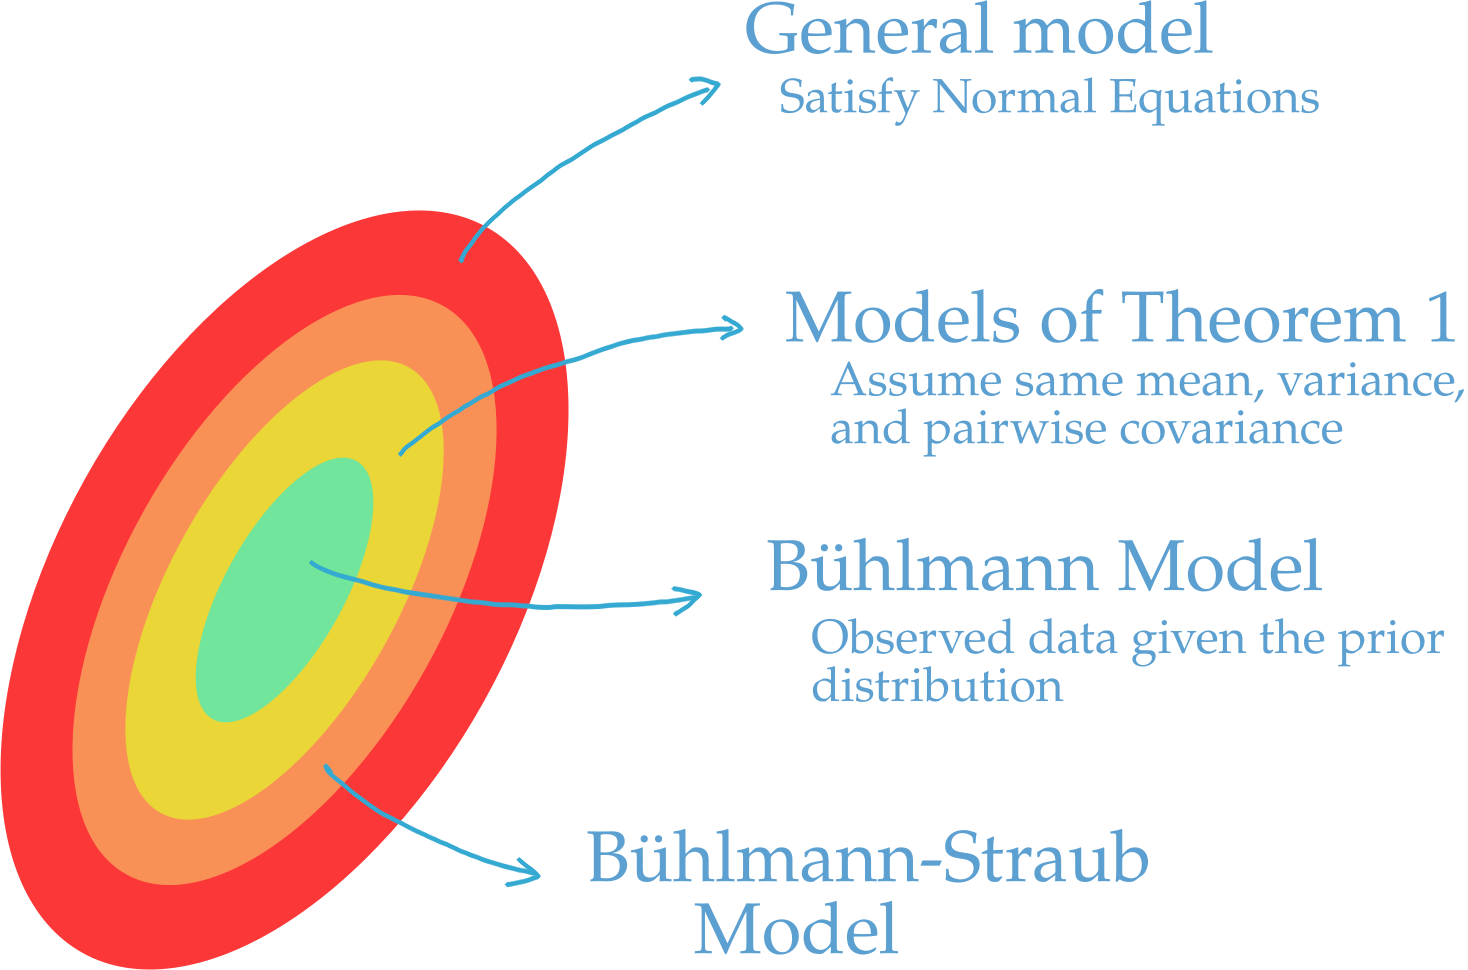
\includegraphics[width=0.65\linewidth]{images/hierarchy-of-cred-models.png}
  \caption{Hierarchy of Credibility Models thus far}
  \label{fig:hierarchy_of_credibility_models_thus_far}
\end{figure*}

Suppose that a total of $n$ groups of past observation,
with $m_j$ being the total number of members of group $j$,
\sidenote{In \citealt{klugman2012}, $m_j$ is called a known \hlnoteb{constant
measuring exposure}, and it may represent
\begin{itemize}
  \item the number of months the policy was in force in past year $j$;
  \item number of individuals in the group in past year $j$; or
  \item the amount of premium income for the policy in past year $j$.
\end{itemize}
}
for $j \in \{ 1, \ldots, n \}$.
Let $Y_{jk}$ denote the claim amount for the $k$-th member of group $j$,
for $k \in \{ 1, \ldots, m_j \}$.
For this generalization, let us assume that $Y_{jk} \mid \Theta$ are iid
for each $j$ and $k$, with
\begin{equation*}
  \mu(\theta) = E[Y_{jk} \mid \Theta = \theta] \quad\text{ and }\quad
  v(\theta) = \Var(Y_{jk} \mid \Theta = \theta).
\end{equation*}
Let the \hldefn{structural parameters} of this model be denoted by
\begin{equation*}
  \mu = E[\mu(\theta)],\quad v = E[v(\theta)], \text{ and }\quad
  a = \Var[\mu(\theta)].
\end{equation*}
Let $X_j$ be the \hlnoteb{average claim amount per member} in year $j$,
\sidenote{This is a rather specific construction of the B\"{u}lhmann-Straub
model. The textbook has a slightly more general construction,
and proves for the most general version of the model.}
i.e.
\begin{equation*}
  X_j = \frac{1}{m_j} \sum_{k=1}^{m_j} Y_{jk}.
\end{equation*}
For practical purposes, \sidenote{This is the usual practice in actuarial firms,
where individual records are not tracked (expensive and time-consuming),
but group records are quite easily tracked.}
suppose we can observe the average claim amount $X_j$ (from the total amount
$m_j X_j$ and the number of members $m_j$), but the individual claims $\{ Y_{jk}
\}_{k=1}^{m_j}$ are not observable.

\begin{thm}[B\"{u}hlmann-Straub Model]\index{B\"{u}hlmann-Straub Model}\label{thm:buhlmann_straub_model}
  With the above assumptions, the B\"{u}hlmann-Straub Model has
  \begin{gather*}
    E[X_j \mid \Theta] = \mu(\Theta),
    \Var(X_j \mid \Theta) = \frac{v(\theta)}{m_j}, \\
    E[X_j] = \mu,\quad
    \Var(X_j) = \frac{v}{m_j} + a,\text{ and } \\
    \Cov(X_i, X_j) = a \text{ for } i \neq j.
  \end{gather*}
\end{thm}

\begin{proof}
  By assumption, $\{Y_{jk} \mid \Theta\}$ is an iid sequence of rvs,
  with
  \begin{equation*}
    \mu(\theta) = E[Y_{jk} \mid \Theta = \theta] \text{ and }
    v(\theta) = \Var(Y_{jk} \mid \Theta = \theta).
  \end{equation*}
  Then since $X_j = \frac{1}{m_j} \sum_{k=1}^{m_j} Y_{jk}$, we have
  \begin{align*}
    E[X_j \mid \Theta = \theta]
    &= E \left[ \frac{1}{m_j} \sum_{k=1}^{m_j} Y_{jk}
      \mid \Theta = \theta \right] \\
    &= \frac{1}{m_j} \sum_{k=1}^{m_j} E [ Y_{jk} \mid \Theta = \theta ]
      \quad\because \text{ linearity of } E \\
    &= \frac{1}{m_j} \sum_{k=1}^{m_j} \mu(\theta)
     = \frac{1}{m_j} m_j \mu(\theta) \\
    &= \mu(\theta),
  \end{align*}
  and
  \begin{align*}
    \Var(X_j \mid \Theta = \theta)
    &= \Var\left( \frac{1}{m_j} \sum_{k=1}^{m_j} Y_{jk}
      \mid \Theta = \theta \right) \\
    &= \frac{1}{m_j^2} \sum_{k=1}^{m_j} \Var(Y_{jk} \mid \Theta = \theta)
      \quad\because \substack{\text{linearity of $\Var$ \&} \\
      \text{ independence of } Y_{jk}}  \\
    &= \frac{1}{m_j^2} m_j v(\theta) = \frac{v(\theta)}{m_j}.
  \end{align*}
  Furthermore,
  \begin{align*}
    E[X_j] &= E[E[X_j \mid \Theta]] \\
           &= E[\mu(\theta)] = \mu \\
    \Var(X_j) &= \Var(E[X_j \mid \Theta]) + E[\Var(X_j \mid \Theta)] \\
              &= \Var(\mu(\theta)) + E \left[ \frac{v(\theta)}{m_j} \right] \\
              &= a + \frac{v}{m_j},
  \end{align*}
  and for $i \neq j$, noticing that $X_i \mid \Theta \coprod X_j \mid \Theta$
  due to the independence of the $(Y_{jk} \mid \Theta)$'s, we have
  \begin{align*}
    \Cov(X_i, X_j)
    &= E[X_i X_j] - E[X_i]E[X_j] \\
    &= E[E[X_i X_j \mid \Theta]] - \mu^2 \\
    &= E[E[X_i \mid \Theta] E[X_j \mid \Theta]] - \mu^2 \\
    &= E[\mu(\theta)^2] - \mu^2 \\
    &= Var(\mu(\theta)) + E[\mu(\theta)]^2 - \mu^2 \\
    &= a + 0 = a.
  \end{align*}
\end{proof}

\begin{thm}[B\"{u}hlmann-Straub Credibility Premium]\index{B\"{u}hlmann-Straub Credibility Premium}\label{thm:buhlmann_straub_credibility_premium}
  The \hlnoteb{B\"{u}hlmann-Straub Credibility Premium} is
  \begin{equation*}
    P = Z \overline{X} + (1 - Z)\mu,
  \end{equation*}
  where
  \begin{equation*}
    Z = \frac{m}{m + \frac{v}{a}}, \quad
    \overline{X} = \sum_{i=1}^{n} \frac{m_i}{m} X_i,\text{ and }\quad
    m = \sum_{i=1}^{n} m_i.
  \end{equation*}
\end{thm}

\begin{proof}
  With \cref{thm:buhlmann_straub_model}, we have
  that the credibility premium is given by
  \begin{equation*}
    P = \hat{\alpha}_0 + \sum_{j=1}^{n} \hat{\alpha}_j X_j,
  \end{equation*}
  by \cref{defn:estimator_for_the_credibility_premium},
  where the $\hat{\alpha}_i$'s are chosen to minimize the mean square error
  \begin{equation*}
    \mathcal{Q}(\alpha_0, \ldots, \alpha_n)
    = E \left[ \left( X_{n+1} - \left[ \alpha_0 + \sum_{j=1}^{n} \alpha_j X_j
      \right] \right)^2 \right]
  \end{equation*}
  as seen in
  \hyperref[thm:general_model_for_credibility_premium]{the general model}.
  We need to figure out what the $\hat{\alpha}_i$'s are.
  In particular, $(\hat{\alpha}_0, \ldots \hat{\alpha}_n)$
  solves the normal equations
  \begin{equation*}
    \begin{cases}
      E[X_{n+1}] = \hat{\alpha}_0 + \sum_{j=1}^{n} \hat{\alpha}_j E[X_i] \\
      \Cov(X_j, X_{n+1}) = \sum_{i=1}^{n} \hat{\alpha}_i \Cov(X_i, X_j) \text{
      for } j \in \{ 1, \ldots, n \}.
    \end{cases}
  \end{equation*}
  Under our assumptions, the equations become
  \begin{gather}
    \mu = \hat{\alpha}_0 + \sum_{j=1}^{n} \hat{\alpha}_j \mu  \tag{$\dagger$}\\
    a = \sum\limits_{\substack{i=1 \\ i \neq j}}^{n}
      \hat{\alpha}_i a + \hat{\alpha}_j \left( \frac{v}{m_j} + a \right)
      \text{ for } j \in \{ 1, \ldots, n \}. \tag{$*$}
  \end{gather}
  Dividing both sides by $a$, we have that $(*)$ becomes
  \begin{equation*}
    1 = \sum_{i=1}^{n} \hat{\alpha}_i + \hat{\alpha}_j \frac{v}{am_j}
  \end{equation*}
  which implies
  \begin{equation}\label{eq:buhlmann_straub_prem_eq1}
    \sum_{i=1}^{n} \hat{\alpha}_i = 1 - \hat{\alpha}_j \frac{v}{am_j}.
  \end{equation}
  Putting this into $(\dagger)$, we get
  \begin{equation*}
    \mu = \hat{\alpha}_0 + \mu \left( 1 - \hat{\alpha}_j \frac{v}{am_j} \right),
  \end{equation*}
  and so
  \begin{equation}\label{eq:buhlmann_straub_prem_eq2}
    \hat{\alpha}_0 = \hat{\alpha}_j \frac{v\mu}{am_j} \implies
    \hat{\alpha}_j = \frac{am_j}{v\mu} \hat{\alpha}_0.
  \end{equation}
  Going back to \cref{eq:buhlmann_straub_prem_eq1}, we have
  \begin{equation*}
    \frac{am}{v\mu} \hat{\alpha}_0
    = \frac{a}{v\mu} \hat{\alpha}_0 \sum_{i=1}^{n} m_j
    = 1 - \frac{1}{\mu} \hat{\alpha}_0
    \implies \hat{\alpha}_0 \left( \frac{am}{v\mu} + \frac{1}{\mu} \right) = 1
  \end{equation*}
  which thus
  \begin{equation*}
    \hat{\alpha}_0 = \frac{1}{\frac{am + v}{v\mu}}
    = \frac{v}{ma + v} \mu
    = \frac{\frac{v}{a}}{m + \frac{v}{a}} \mu.
  \end{equation*}
  Consequently, going back to \cref{eq:buhlmann_straub_prem_eq2} gives
  \begin{equation*}
    \hat{\alpha}_j = \frac{am_j}{v\mu} \cdot \frac{v\mu}{ma +v}
    = \frac{m_j}{m + \frac{v}{a}} \text{ for all } j \in \{1, \ldots, n\}.
  \end{equation*}
  Thus the B\"{u}hlmann-Straub credibility premium is
  \begin{align*}
    P &= \hat{\alpha}_0 + \sum_{i=1}^{n} \hat{\alpha}_i X_i \\
      &= \frac{\frac{v}{a}}{m + \frac{v}{a}} \mu + \sum_{i=1}^{n}
        \frac{m_j}{m+\frac{v}{a}} X_i \\
      &= \frac{m}{m + \frac{v}{a}} \sum_{i=1}^{n} \frac{m_i}{m} X_i
        + \frac{\frac{v}{a}}{m + \frac{v}{a}} \mu \\
      &= Z \overline{X} + (1 - Z) \mu,
  \end{align*}
  where
  \begin{equation*}
    Z = \frac{m}{m + \frac{v}{a}}, \quad
    \overline{X} = \sum_{i=1}^{n} \frac{m_i}{m} X_i,\text{ and }\quad
    m = \sum_{i=1}^{n} m_i,
  \end{equation*}
  as desired.
\end{proof}

\begin{procedure}[Finding the B\"{u}lmann Straub Credibility Premium]\label{procedeure:finding_the_buhlmann_straub_credibility_premium}
  \cref{thm:buhlmann_straub_model} and
  \cref{thm:buhlmann_straub_credibility_premium}
  shows us how to calculate the credibility premium.
  \begin{enumerate}
    \item Define an appropriate $X_j$.
    \item Find $\mu(\theta) = E[X_j \mid \Theta]$
      and $\frac{v(\theta)}{m_j} = \Var(X_j \mid \Theta)$.
    \item Find the structural parameters
      \begin{equation*}
        \mu = E[\mu(\Theta)]
        v = E[v(\Theta)] \text{ and }
        a = \Var(\mu(\Theta)).
      \end{equation*}
    \item Calculate $Z, \overline{X}$ and $m$.
    \item Put everything into
      \begin{equation*}
        P = Z \overline{X} + (1 - Z) \mu.
      \end{equation*}
  \end{enumerate}
  Step 1 is the main boss of the challenge.
  If one can figure out what the problem needs us to set $X_j$ as,
  then half the battle is done.
\end{procedure}

\begin{eg}
  In year $j$, for $j \in \{1, \ldots, n \}$, there are $m_j$ members
  and let $N_j$ be the number of claims, where
  \begin{itemize}
    \item $N_j \mid \Theta = \theta \sim \Poi(m_j \theta)$ are independent; and
    \item $\Theta \sim \Gam(\alpha, \beta)$.
  \end{itemize}
  Determine the B\"{u}hlmann-Straub Credibility Premium
  for the average number of claims in year $n + 1$ per member.
\end{eg}

\begin{solution}
  We want to find the credibility premium for
  \begin{equation*}
    X_{n+1} = \frac{N_{n+1}}{m_{n+1}}.
  \end{equation*}
  Thus, for $j \in \{ 1, \ldots, n \}$, let
  \begin{equation*}
    X_j = \frac{N_j}{m_j}.
  \end{equation*}
  Then
  \begin{align*}
    \mu(\theta) &= E[X_j \mid \Theta = \theta]
                 = E \left[ \frac{N_j}{m_j} \mid \Theta = \theta \right] \\
                &= \frac{1}{m_j} E [ N_j \mid \Theta = \theta ] \\
                &= \frac{1}{m_j} m_j \theta = \theta,
  \end{align*}
  and
  \begin{align*}
    \frac{v(\theta)}{m_j} = \Var(X_j \mid \Theta = \theta)
    &= \frac{1}{m_j^2} \Var(N_j \mid \Theta = \theta) \\
    &= \frac{1}{m_j^2} m_j \theta = \frac{\theta}{m_j}.
  \end{align*}
  Moving along,
  \begin{align*}
    \mu &= E[X_j] = E[E[X_j \mid \Theta]] = E[\mu(\Theta)]
      = E[\Theta] = \alpha\beta \\
    v &= E[v(\Theta)] = E[\Theta] = \alpha\beta \\
    a &= \Var(\mu(\Theta)) = \Var(\Theta) = \alpha\beta^2.
  \end{align*}
  Thus
  \begin{equation*}
    Z = \frac{m}{m + \frac{v}{a}} = \frac{m}{m + \beta^{-1}},
  \end{equation*}
  and so
  \begin{equation*}
    P = \frac{m}{m + \beta^{-1}} \overline{X} + \frac{\beta^{-1}}{m +
    \beta^{-1}} \alpha\beta.
  \end{equation*}
\end{solution}

\begin{note}
  \begin{enumerate}
    \item It is not surprise to see that if we fix $m_j = 1$
      for all $j \in \{1, \ldots, n\}$, then we get back into the
      \hyperref[thm:buhlmann_credibility_premium]{B\"{u}hlmann Model}.
  \end{enumerate}
\end{note}

% section buhlmann_straub_model (end)

\newpage
\section{Exact Credibility}%
\label{sec:exact_credibility}
% section exact_credibility

\marginnote{
\begin{textbook}
  \citealt{klugman2012} Section 18.7 (pg 397)
\end{textbook}
}

Recall that in \cref{eg:a_poisson_gamma_example_for_buhlmann_credibility},
we saw that the B\"{u}hlmann credibility premium agreed with
the Bayesian premium. However, in
\cref{eg:disagreement_of_buhlmann_credibility_premium_and_bayesian_premium},
we saw that they disagreed.
One cannot help but wonder when exactly does the agreement happen,
and when does it not.

Recall that in \cref{thm:general_model_for_credibility_premium},
the credibility premium is designed to be the best linear approximation
to the Bayesian premium.

\begin{defn}[Exact Credibility]\index{Exact Credibility}\label{defn:exact_credibility}
  When the credibility premium from
  \cref{thm:general_model_for_credibility_premium}
  and the Bayesian premium coincide, we describe this situation as
  \hlnoteb{exact credibility}.
\end{defn}

\begin{note}
  In particular, when exact credibility occurs, we have that
  \begin{equation*}
    \mathcal{Q}(\alpha_0, \ldots, \alpha_n) = 0.
  \end{equation*}
\end{note}

The following is a result that illustrates the occurrence of exact probability.

\begin{propo}[Exact Credibility when Observations Belong to the Linear Exponential Family]\label{propo:exact_credibility_when_observations_belong_to_the_linear_exponential_family}
  Suppose $\{ X_i \}_{i=1}^{n}$ is an iid sequence that belongs to the linear
  exponential family, that is
  \begin{equation*}
    f_{X_i \mid \Theta}(x_i \mid \theta) = \frac{p(x_i) e^{r(\theta)
    x_i}}{q(\theta)},
  \end{equation*}
  where $p$ is a function of $x_i$, and $r, q$ are functions of $\theta$.
  Furthermore, suppose that $\Theta$ is a
  \hyperref[defn:conjugate_prior_distribution]{conjugate prior distribution}
  with density
  \begin{equation*}
    \pi(\theta) = \frac{q(\theta)^{-k} e^{\mu k r(\theta)} r'(\theta)}{c(\mu,
    k)},
  \end{equation*}
  where $c(\mu, k)$ is a constant determined by $\mu$ and $k$.
  Also, suppose that $\theta_0 \leq \Theta \leq \theta_1$, and that
  \begin{equation*}
    \frac{\pi(\theta_0 \mid x_1, \ldots, x_n)}{r'(\theta_0)}
    = \frac{\pi(\theta_1 \mid x1, \ldots, x_n)}{r'(\theta_1)}.
  \end{equation*}
  Then the Bayesian premium is the credibility premium, i.e.
  \begin{equation*}
    E[X_{n+1} \mid X_1, \ldots, X_n] = \alpha_0 + \sum_{i=1}^{n} \alpha_i X_i,
  \end{equation*}
  where $(\alpha_0, ..., \alpha_n)$ is as in
  \cref{thm:general_model_for_credibility_premium}.
\end{propo}

The proof of the above theorem will not be included here,
but one can read the textbook on page 398. \cite{klugman2012}

% section exact_credibility (end)

% chapter greatest_accuracy_credibility (end)

\chapter{Empirical Bayes Parameter Estimation}%
\label{chp:empirical_bayes_parameter_estimation}
% chapter empirical_bayes_parameter_estimation

\section{Introduction}%
\label{sec:introduction}
% section introduction

In \cref{chp:greatest_accuracy_credibility}, we used the Bayesian or
credibility premium to incorporate past data into our prospective premium.
One flaw of this approach is that it strongly depends on assumed distributions,
in particular for $f_{X_j \mid \Theta}$ and $\pi$.
More realistically, it is not necessary easy to know, for instance,
values for $\alpha$ and $\beta$ if $\Theta \sim \Gam(\alpha, \beta)$.

In general, these unknown parameters are associated with the \hldefn{structure
density} $\pi(\theta)$, hence the name \hldefn{structural parameters} for the
values
\begin{equation*}
  \mu = E[\mu(\Theta)], v = E[v(\Theta)] \text{ and } a = \Var(\mu(\Theta)).
\end{equation*}
We may need to use the data at hand to estimate the structural parameters.
This approach is known as the \hldefn{empirical Bayes estimation}.
\sidenote{It is important to note that this is different from looking for the
posterior distribution.

Furthermore, in standard Bayesian methods, the prior distribution is strictly
assumed to be fixed before any data is observed.}

There are a total of 3 cases of which we shall look into:
\begin{itemize}
  \item \hlnoted{Non-parametric estimation}
    -- where both $f_{X_i \mid \Theta}$ and $\pi$ are unspecified;
  \item \hlnoted{Semi-parametric estimation}
    -- where $f_{X_i \mid \Theta}$ is assumed to be of a parametric form but
    $\pi$ is unspecified; and
  \item \hlnoted{Parametric estimation}
    -- where both $f_{X_i \mid \Theta}$ and $\pi$ are both assumed to be of
    parametric form.
\end{itemize}

\begin{note}
  \begin{itemize}
    \item The decision as to whether to select a parametric model or not
      depends partially on the situation at hand
      and partially on the judgement and knowledge
      of the person performing the analysis.

    \item Non-parametric models have the advantage of being appropriate
      for a wide variety of situations, a fact that actually makes it
      the easiest of the 3 to work with.
  \end{itemize}
\end{note}

Let us first set up the most general model for tackling these problems.

\begin{defn}[General Model Setting for Empirical Bayes Parameter Estimation]\label{defn:general_model_setting_for_empirical_bayes_parameter_estimation}
  Consider $r$ groups of policies. For $i \in \{1, \ldots, r \}$, let

  \begin{tabular}{c l}
  $n_i$       & be the number of years of observations for group $i$, \\
  $m_{ij}$    & be the number of members/\hldefn{exposure units} \\
              & for group $i$ in year $j$, for $j \in \{ 1, \ldots, n_i \}$ \\
  $\vec{m}_i$ & vector for the number of exposure units for group $i$, \\
              & i.e. $\vec{m}_i = (m_{i1}, \ldots, m_{in_i})$, \\
  $m_i$       & be the total number of exposure for group $i$, i.e. \\
              & $m_i = \sum\limits_{j=1}^{n_j} m_{ij}$, \\
  $m$         & total number of exposure units for all groups, i.e. \\
              & $m = \sum\limits_{i=1}^{r} m_i = \sum\limits_{i=1}^{r}
                \sum\limits_{j=1}^{n_i} m_{ij}$, \\
  $X_{ij}$    & average claim experience (amount/number) of claims \\
              & for group $i$ in year $j$, for $j \in \{1, \ldots, n_i\}$, \\
  $\vec{X}_i$ & vector for the average (amount/number) of claims \\
              & for group $i$, i.e. $\vec{X}_i = (X_{i1}, \ldots, X_{in_i})$, \\
  $\overline{X}_i$ & past average claim experience for group $i$, i.e. \\
                   & $\overline{X}_i = \frac{1}{m_i} \sum\limits_{j=1}^{n_i}
                    m_{ij} X_{ij}$ \\
  $\overline{X}$ & average claim experience for all groups, i.e. \\
                 & $\overline{X} = \frac{1}{m} \sum\limits_{i=1}^{r} 
                    m_i \overline{X}_i = \frac{1}{m} \sum\limits_{i=1}^{r}
                    \sum\limits_{j=1}^{n_i} m_{ij} X_{ij}$.
  \end{tabular}

  Furthermore, in this chapter, we shall
  \begin{itemize}
    \item denote the unknown risk parameter for group $i$ as $\Theta_i$,
    \item and assume that $\{ \Theta_i \}_{i=1}^{r}$ is an iid sequence
      with common density $\pi_{\Theta_i}$;
    \item assume the experience is different groups are independent
      (across groups), i.e. 
      $\vec{X}_i \coprod \vec{X}_j$ for $i \neq j \in \{1, \ldots, r\}$;
    \item assume $\{ X_{ij} \mid \Theta_i \}_{i=1}^{r}$ are independent
      (across periods), with density $f_{X_{ij} \mid \Theta}$, where
      \begin{equation*}
        E[X_{ij} \mid \Theta_i] \mu(\Theta_i) \quad
        \Var(X_{ij} \mid \Theta_i) = \frac{v(\Theta_i)}{m_{ij}}.
      \end{equation*}
  \end{itemize}
\end{defn}

% TODO include diagram from module 6

\begin{note}
  In the last of our assumptions above,
  notice that $E[X_{ij} \mid \Theta_i] = \mu(\Theta_i)$
  does not depend on the period.
\end{note}

% section introduction (end)

\section{Non-Parametric Estimation}%
\label{sec:non_parametric_estimation}
% section non_parametric_estimation

Let us now try to use this approach
to estimate the structural parameters.
But before that, a lemma.

\begin{lemma}[Weaker Version of Sample Mean and Variance]\label{lemma:weaker_version_of_sample_mean_and_variance}
  Let
  \begin{equation*}
    \overline{Y} = \frac{1}{n} \sum_{i=1}^{n} Y_i
  \end{equation*}
  and
  \begin{equation*}
    \overline{Y} \mid \Theta
    = \left[ \left( \frac{1}{n} \sum_{i=1}^{n}
      Y_i \right) \mid \Theta \right]
    = \frac{1}{n} \sum_{i=1}^{n} (Y_i \mid \Theta).
  \end{equation*}
  Then
  \begin{enumerate}
    \item If $\{ Y_i \}_{i=1}^{n}$ are \hlnotec{independent}
      and have \hlnotec{common mean} $E[Y_i] = \mu$
      and \hlnotec{common variance} $\Var(Y_i) = v$, then
      \begin{equation*}
        E[\overline{Y}] = \mu,\quad
        E \left[ \frac{1}{n-1} \sum_{i=1}^{n} (Y_i - \overline{Y})^2 \right] =
        v.
      \end{equation*}

    \item If $\{ Y_i \mid \Theta \}_{i=1}^{n}$ are \hlnotec{independent} and
      have \hlnotec{common conditional mean} $E[Y_i \mid \Theta] = \mu(\Theta)$,
      \hlnotec{common conditional variance} $\Var(Y_i \mid \Theta) = v(\Theta)$,
      then
      \begin{gather*}
        E[\overline{Y} \mid \Theta] = \mu(\Theta) \\
        E \left[ \frac{1}{n-1} \sum_{i=1}^{n}
          (Y_i - \overline{Y})^2 \mid \Theta \right] = v(\Theta).
      \end{gather*}
  \end{enumerate}
\end{lemma}

\begin{ex}
  Prove \cref{lemma:weaker_version_of_sample_mean_and_variance}.
\end{ex}

In the \hyperref[defn:the_buhlmann_model]{B\"{u}hlmann model},
we have that
\begin{itemize}
  \item $n_i = n$ for all $i \in \{1, \ldots, r\}$, i.e.
    we have the same number of years of experience for all groups;
  \item $m_{ij} = 1$ for all $i \in \{1, \ldots, r\},\, j \in \{1, \ldots, n\}$,
    i.e. only 1 member in each group in each year; and
  \item that $\{ X_{ij} \mid \Theta_i \}_{j=1}^{n}$ are iid.
\end{itemize}
Under
\cref{defn:general_model_setting_for_empirical_bayes_parameter_estimation},
we have
\begin{itemize}
  \item $m_i = \sum_{j=1}^{n} m_{ij} = n$ ;
  \item $m = \sum_{i=1}^{r} m_i = nr$ ;
  \item $\overline{X}_i = \frac{1}{m_i} \sum_{j=1}^{n} m_{ij} X_{ij} =
    \frac{1}{n} \sum_{j=1}^{n} X_{ij}$; and
  \item $\overline{X} = \frac{1}{m} \sum_{i=1}^{r} \sum_{j=1}^{n} m_{ij} X_{ij}
    = \frac{1}{nr} \sum_{i=1}^{r} \sum_{j=1}^{n} X_{ij}$.
\end{itemize}

\begin{propo}[Non-Parametric Estimation for B\"{u}hlmann Model]\label{propo:non_parametric_estimation_for_buhlmann_model}
  For a \hyperref[defn:the_buhlmann_model]{B\"{u}hlmann model},
  we have that
  \begin{enumerate}
    \item an unbiased estimator for $\mu$ is $\hat{\mu} = \overline{X}$ ;
    \item an unbiased estimator for $v$ is
      \begin{equation*}
        \hat{v} = \frac{1}{r} \sum_{i=1}^{r} \hat{v}_i,
      \end{equation*}
      where
      \begin{equation*}
        \hat{v}_i = \frac{1}{n-1} \sum_{j=1}^{n} (X_{ij} - \overline{X}_i)^2,
      \end{equation*}
      which is also an unbiased estimator for $v$.
    \item an unbiased estimator for $a$ is
      \begin{equation*}
        \hat{a} = \frac{1}{r-1} \sum_{i=1}^{r} (\overline{X}_i - \overline{X})^2
        - \frac{\hat{v}}{n}.
      \end{equation*}
  \end{enumerate}
\end{propo}

\begin{ex}
  Use \cref{lemma:weaker_version_of_sample_mean_and_variance} to
  prove \cref{propo:non_parametric_estimation_for_buhlmann_model}.
  This should be an easy and straightforward exercise.
\end{ex}

\begin{note}
  \begin{itemize}
    \item We use $\hat{Z}$ to denote the estimated credibility factor.
    \item It is important to note that $\hat{Z}$ is usually not
      an unbiased estimator for $Z$.
    \item If $\hat{a} \leq 0$, we set $\hat{a} = \hat{Z} = 0$.
    \item We let the \hldefn{Estimated Bühlmann premium} for group $i$ be
      \begin{equation*}
        \hat{Z} \overline{X}_i + (1 - \hat{Z}) \hat{\mu}.
      \end{equation*}
  \end{itemize}
\end{note}

\begin{procedure}[Finding an Estimated B\"{u}hlmann Premium]\label{procedure:finding_an_estimated_buhlmann_premium}
  \begin{enumerate}
    \item Use \cref{propo:non_parametric_estimation_for_buhlmann_model}
      to estimate the structural parameters
      $\hat{\mu},\, \hat{v}$, and $\hat{a}$.
    \item Use \cref{thm:buhlmann_credibility_premium}
      with the structural parameters to estimate the B\"{u}hlmann premium.
  \end{enumerate}
\end{procedure}

\begin{eg}
  In the B\"{u}hlmann model, suppose that:
  \begin{itemize}
    \item there are 2 groups with 3 years of experience each; and
    \item losses are $\vec{X}_1 = (3, 5, 7)$ and $\vec{X}_2 = (6, 12, 9)$.
  \end{itemize}
  Estimate the B\"{u}hlmann credibility premium for each group in year 4.
\end{eg}

\begin{solution}
  We are given that $r = 2$ and $n = 3$.
  Then since
  \begin{equation*}
    \overline{X}_1 = \frac{3+5+7}{3} = 5 \text{ and }
    \overline{X}_2 = \frac{6+12+9}{3} = 9,
  \end{equation*}
  we have
  \begin{equation*}
    \hat{\mu} = \frac{5+9}{2} = 7.
  \end{equation*}
  Furthermore,
  \begin{gather*}
    \hat{v}_1 = \frac{1}{3-1}[ (3-5)^2 + (5-5)^2 + (7-5)^2 ] = 4 \\
    \hat{v}_2 = \frac{1}{3-1}[ (6-9)^2 + (12-9)^2 + (9-9)^2 ] = 9,
  \end{gather*}
  and so
  \begin{equation*}
    \hat{v} = \frac{1}{2} (4 + 9) = \frac{13}{2}.
  \end{equation*}
  Lastly,
  \begin{equation*}
    \hat{a} = \frac{1}{2-1} [(5-7)^2 + (9-7)^2] - \frac{\frac{13}{2}}{3}
          = \frac{35}{6}.
  \end{equation*}
  Thus the estimated Bühlmann credibility factor is
  \begin{equation*}
    \hat{Z} = \frac{n}{n + \frac{\hat{v}}{\hat{a}}}
    = \frac{3}{3 + \frac{\frac{13}{2}}{\frac{35}{6}}}
    = \frac{35}{48}.
  \end{equation*}
  It follows that the estimated Búhlmann credibility premium
  for group 1 and 2 are
  \begin{gather*}
    \hat{Z} \overline{X}_1 + (1 - \hat{Z}) 7 = \frac{133}{24} \\
    \hat{Z} \overline{X}_2 + (1 - \hat{Z}) 7= \frac{203}{4},
  \end{gather*}
  respectively.
\end{solution}

\newthought{In the} \hyperref[thm:buhlmann_straub_model]{Bühlmann-Straub model},
the notation mostly follows what is in
\cref{defn:general_model_setting_for_empirical_bayes_parameter_estimation}.

\begin{propo}[Non-Parametric Estimation for Bühlmann-Straub Model]\label{propo:non_parametric_estimation_for_buhlmann_straub_model}
  For a Bühlmann-Straub model, we have that
  \begin{enumerate}
    \item an unbiased estimator for $\mu$ is $\hat{\mu} = \overline{X}$ ;
    \item an unbiased estimator for $v$ is
      \begin{equation*}
        \hat{v} = \frac{1}{\sum_{i=1}^{r} (n_i - 1)}
          \sum_{i=1}^{r} (n_i - 1) \hat{v}_i,
      \end{equation*}
      where
      \begin{equation*}
        \hat{v}_i = \frac{1}{n_i - 1} \sum_{j=1}^{n_i}
          m_{ij} (X_{ij} - \overline{X}_i)^2,
      \end{equation*}
      which is also an unbiased estimator for $v$; and
    \item an unbiased estimator for $a$ is
      \begin{equation*}
        \hat{a} = \frac{m}{m^2 - \sum_{i=1}^{r} m_i^2} \left( 
          \sum_{i=1}^{r} m_i (\overline{X}_i - \overline{X})^2 - (r-1)\hat{v}
        \right)
      \end{equation*}
  \end{enumerate}
\end{propo}
\marginnote{The proof of
\cref{propo:non_parametric_estimation_for_buhlmann_straub_model} is also a
follow your nose proof, but I shall include it here.}

\begin{proof}
  \hlwarn{To be added.}
\end{proof}

\begin{note}[Estimated Bühlmann-Straub Premium]\label{note:estimated_buhlmann_straub_premium}
  \begin{itemize}
    \item With the Bühlmann-Straub model, we can actually even
      estimate the premium for \hlnotec{each member group $i$},
      which is given by
      \begin{equation*}
        \hat{Z}_i \overline{X}_i + (1 - \hat{Z}_i) \hat{\mu},
      \end{equation*}
      where the \hldefn{Estimated Bühlmann-Straub Credibility Factor}
      for group $i$ is
      \begin{equation*}
        \hat{Z}_i = \frac{m_i}{m_i + \frac{\hat{v}}{\hat{a}}}.
      \end{equation*}
    \item The estimated Bühlmann-Straub premium for \hlnotec{the whole group $i$}
      in year $n_i + 1$ is
      \begin{equation*}
        m_{i (n_i+1)} \left(\hat{Z}_i \overline{X}_i + (1 - \hat{Z})\hat{\mu}\right).
      \end{equation*}
    \item Again, when $\hat{a} \leq 0$, we set $\hat{a} = \hat{Z} = 0$.
  \end{itemize}
\end{note}

\begin{procedure}[Finding an Estimated Bühlmann-Straub Premium]\label{procedure:finding_an_estimated_buhlmann_straub_premium}
  \begin{enumerate}
    \item Use \cref{propo:non_parametric_estimation_for_buhlmann_straub_model}
      to find the estimated structural parameters $\hat{\mu},\, \hat{v}$, and
      $\hat{a}$.
    \item Use \cref{note:estimated_buhlmann_straub_premium}
      to calculate the appropriate premiums for the appropriate setting.
  \end{enumerate}
\end{procedure}

\paragraph{Another estimator for $\mu$}
There is another estimator of which we can estimate $\mu$.

\begin{defn}[Total Loss of All Groups]\label{defn:total_loss_of_all_groups}
  The \hlnoteb{total loss (TL)} of all groups in the past is defined as
  \begin{equation*}
    \TL = \sum_{i=1}^{r} m_i \overline{X}_i.
  \end{equation*}
\end{defn}

\begin{defn}[Total Premium of All Groups]\label{defn:total_premium_of_all_groups}
  If we \hlnotec{charged credibility premium in the past}, then we define
  the \hlnoteb{total premium (TP)}  of all groups as
  \begin{equation*}
    \TP = \sum_{i=1}^{r} m_i \left( \hat{Z}_i \overline{X}_i + (1 -
    \hat{Z}_i)\mu \right).
  \end{equation*}
\end{defn}

\begin{propo}[Credibility Weighted Average]\index{Credibility Weighted Average}\label{propo:credibility_weighted_average}
  If $\TL = \TP$, then
  \begin{equation*}
    \hat{\mu} = \frac{1}{\sum_{i=1}^{r} \hat{Z}_i}
      \sum_{i=1}^{r} \hat{Z}_i \overline{X}_i \quad,
  \end{equation*}
  called a \hlnoteb{credibility weighted average},
  is an unbiased estimator for $\mu$.
\end{propo}

\begin{ex}
  Prove \cref{propo:credibility_weighted_average}.
  Again, this is an easy exercise.
\end{ex}

\begin{eg}[Example for Estimated Bühlmann-Straub Premium]
  Past claim data of 2 groups is given as follows.
  \begin{table}[ht]
    \centering
    \caption{Past claim data for Example for Estimated Bühlmann-Straub Premium}
    \label{table:past_claim_data_for_example_for_estimated_buhlmann_straub_premium}
    \begin{tabular}{l | c c c c}
    Year                         & 1   & 2    & 3   & 4 \\
    \hline
    Total claims in group 1      &     & 750  & 600 & \\
    Number of members in group 1 &     & 3    & 2   & 4 \\
    \hline
    Total claims in group 2      & 975 & 1200 & 900 & \\
    Number of members in group 2 & 5   & 6    & 4   & 5
    \end{tabular}
  \end{table}
  \begin{enumerate}
    \item Calculate the unbiased estimates for $\mu$, $v$ and $a$
      in the Bühlmann-Straub model.
    \item Determine the Bühlmann-Straub premium for each group in year 4.
    \item Redo part (2) if $\mu$ is estimated
      by the credibility weighted average.
  \end{enumerate}
\end{eg}

\begin{solution}
  \begin{enumerate}
    \item Note
      \begin{equation*}
        r = 2,\quad n_1 = 2,\quad n_2 = 3.
      \end{equation*}
      Furthermore, we are given that
      \begin{gather*}
        m_{11} X_{11} = 750\quad m_{12} X_{12} = 600 \\
        m_{21} X_{21} = 975\quad m_{22} X_{22} = 1200\quad m_{23} X_{23} = 900.
      \end{gather*}
      Now
      \begin{align*}
        \overline{X}_1 &= \frac{750 + 600}{3 + 2} = 270 \\
        \overline{X}_2 &= \frac{975 + 1200 + 900}{5 + 6 + 4} = 205.
      \end{align*}
      Thus
      \begin{equation*}
        \hat{\mu} = \overline{X} = \frac{5(270) + 15(205)}{5 + 15} = 221.25.
      \end{equation*}
      Further,
      \begin{align*}
        \hat{v}_1 &= \frac{1}{2-1} \left[ 3 \left( \frac{750}{3} - 270 \right)^2
            + 2 \left( \frac{600}{2} - 270 \right)^2 \right]
            = 3000 \\
        \hat{v}_2 &= \frac{1}{3-1} \left[ 5 \left( \frac{975}{5} - 205 \right)^2
            + 6 \left( \frac{1200}{6} - 205 \right)^2 \right. \\
            &\quad\left.+ 4 \left( \frac{900}{4} - 205 \right)^2 \right]
            = 1125,
      \end{align*}
      and so
      \begin{align*}
        \hat{v} = \frac{1}{(2 - 1) + (3 - 1)} \left[ 
          (2 - 1) 3000 + (3 - 1) 1125
        \right] = 1750.
      \end{align*}
      Finally,
      \begin{align*}
        a &= \frac{20}{20^2 - 5^2 - 15^2} \left[
          5 \left( 270 - 221.25 \right)^2 + 15 (205 - 221.25)^2 \right. \\
          &\quad\left.- (2-1) 1750 \right] = 1879.17.
      \end{align*}

    \item It follows that
      \begin{equation*}
        \hat{Z}_1 = \frac{5}{5 + \frac{\hat{v}}{\hat{a}}} = 0.843 \text{ and }
        \hat{Z}_2 = \frac{15}{15 + \frac{\hat{v}}{\hat{a}}} = 0.9415.
      \end{equation*}
      Thus the estimated Bühlmann-Straub premium for group 1 and 2 are
      \begin{align*}
        4 [ \hat{Z}_1 \overline{X}_1 + (1 - \hat{Z}_1) \hat{\mu} ] &= 1049.38 \\
        5 [ \hat{Z}_2 \overline{X}_2 + (1 - \hat{Z}_2) \hat{\mu} ] &= 1029.75,
      \end{align*}
      respectively.

    \item If we estimate $\mu$ by the credibility weighted average, then
      \begin{equation*}
        \hat{\mu} = \frac{\hat{Z}_1 \overline{X}_1 + \hat{Z}_2
        \overline{X}_2}{\hat{Z}_1 + \hat{Z}_2} = 235.7061.
      \end{equation*}
      Thus the estimated Bühlmann-Straub premium for group 1 and 2,
      using the credibility weighted average estimator of $\mu$,
      are
      \begin{align*}
        4 [ \hat{Z}_1 \overline{X}_1 + (1 - \hat{Z}_1) \hat{\mu} ] &= 1058.44 \\
        5 [ \hat{Z}_2 \overline{X}_2 + (1 - \hat{Z}_2) \hat{\mu} ] &= 1033.98,
      \end{align*}
      respectively.
  \end{enumerate}
\end{solution}

% section non_parametric_estimation (end)

\section{Semi-Parametric Estimation}%
\label{sec:semi_parametric_estimation}
% section semi_parametric_estimation

\marginnote{
\begin{textbook}
  \citealt{klugman2012} Section 19.3 (pg 428)
\end{textbook}
}

Recall that the semi-parametric approach is when we assume that $f_{X_{ij} \mid
\Theta}$ is known.

In semi-parametric estimation,
some \hlnotee{relationship} between $\mu,\, v$ and $a$ is established
which makes estimation simpler.

\begin{procedure}[Relationship between Structural Parameters in Semi-Parameteric Estimation]\label{procedure:relationship_between_structural_parameters_in_semi_parameteric_estimation}
  \begin{enumerate}
    \item Find $\mu(\Theta)$ and $v(\Theta)$.
    \item Find $\mu, v, a$ and see if there is
      some relationship between these structural parameters.
  \end{enumerate}
\end{procedure}

\begin{eg}[Poisson Frequency Model for Semi-Parametric Estimation]
  Suppose $m_{ij} X_{ij} \mid \Theta_i \sim \Poi(m_{ij} \Theta_i)$.
  Find a relationship between the structural parameters, if any.
\end{eg}

\begin{solution}
  First, we have
  \begin{align*}
    \mu(\theta_i) &= E[X_{ij} \mid \Theta_i = \theta_i]
           = \frac{1}{m_{ij}} E [m_{ij} X_{ij} \mid \Theta_i = \theta_i]
           = \frac{1}{m_{ij}} m_{ij} \theta_i = \theta_i \\
    v(\theta_i) &= m_{ij} \Var(X_{ij} \mid \Theta_i = \theta_i)
           = \frac{m_{ij}}{m_{ij}^2} \Var(m_{ij}X_{ij}
             \mid \Theta_i = \theta_i) \\
          &= \frac{1}{m_{ij}} m_{ij} \theta_i = \theta_i.
  \end{align*}
  It's rather clear at this point that $v(\theta_i) = \mu(\theta_i)$
  and so $\mu = v$.
\end{solution}

\begin{eg}[Binomial Frequency Model for Semi-Parametric Estimation]
  Suppose $m_{ij} X_{ij} \mid \Theta_i \sim \Bin(m_{ij}, \Theta_i)$.
  Find a relationship between the structural parameters, if any.
\end{eg}

\begin{solution}
  First, we have
  \begin{align*}
    \mu(\theta_i) &= E[X_{ij} \mid \Theta_i = \theta_i]
           = \frac{1}{m_{ij}} m_{ij} \theta_i = \theta_i \\
    v(\theta_i) &= m_{ij} \Var(X_{ij} \mid \Theta_i = \theta_i)
           = \frac{1}{m_{ij}} m_{ij} \theta_i (1 - \theta_i)
           = \theta_i (1 - \theta_i).
  \end{align*}
  Thus
  \begin{align*}
    \mu &= E[\mu(\Theta_i)] = E[\Theta_i] \\
    v &= E[v(\Theta_i)] = E[\Theta_i - \Theta_i^2] = \mu - \Var(\Theta_i) -
        \mu^2 \\
    a &= \Var(\mu(\Theta_i)) = E[\Theta_i^2] - \mu^2.
  \end{align*}
\end{solution}

\begin{eg}[Exponential Severity Model for Semi-Parametric Estimation]
  Suppose $m_{ij} = 1$ for all $i, j$
  and $X_{ij} \mid \Theta_i \sim \Exp(\Theta_i)$.
  Find a relationship between the structural parameters, if any.
\end{eg}

\begin{solution}
  First, we have
  \begin{align*}
    \mu(\theta_i) &= E[X_{ij} \mid \Theta_i = \theta_i] = \theta_i \\
    v(\theta_i) &= \Var(X_{ij} \mid \Theta_i = \theta_i) = \theta_i^2.
  \end{align*}
  So
  \begin{align*}
    \mu &= E[\mu(\Theta_i)] = E[\Theta_i] \\
    v &= E[v(\Theta_i)] = E[\Theta_i^2] = \Var(\Theta_i) + \mu^2 \\
    a &= \Var(\mu(\Theta_i)) = \Var(\Theta_i) = v - \mu^2.
  \end{align*}
  Thus, in particular,
  \begin{equation*}
    \hat{a} = \hat{v} - \hat{\mu}^2.
  \end{equation*}
\end{solution}

\begin{eg}[Using Semi-Parametric Approach for Estimation]
  In the past year, the distribution of automobile insurance policyholders
  by number of claims is given by
  \cref{table:distribution_of_automobile_insurance_policy_holders_by_number_of_claims}.
  \begin{table}[ht]
    \centering
    \caption{Distribution of Automobile Insurance Policy Holders by Number of
    Claims}
    \label{table:distribution_of_automobile_insurance_policy_holders_by_number_of_claims}
    \begin{tabular}{c c}
    Number of claims & Number of policyholders \\
    \hline
    0                & 1563 \\
    1                & 271 \\
    2                & 32 \\
    3                & 7 \\
    4                & 2 \\
    \hline
    Total            & 1875
    \end{tabular}
  \end{table}
  Assume a (conditional) \hlnotec{Poisson} distribution for
  the number claims for each policy.

  For each policyholder, obtain a credibility estimate for
  the number of claims next year based on the past year's experience.
\end{eg}

\begin{solution}
  Note that we have that each of the policyholders has a well-defined
  risk parameter in this case, and so
  \begin{equation*}
    r = 1875 \quad m_{ij} = 1.
  \end{equation*}
  Also, since this data is from the previous year, $n_i = 1$.
  \sidenote{Ayy! We're in the Bühlmann model!}

  We are given that $X_{ij} \mid \Theta_i \sim \Poi(\Theta_i)$.
  So
  \begin{align*}
    \mu(\theta_i) &= E[X_{ij} \mid \Theta_i = \theta_i] = \theta_i \\
    v(\theta_i) &= \Var(X_{ij} \mid \Theta_i = \theta_i) = \theta_i.
  \end{align*}
  Thus
  \begin{equation*}
    \mu = E[\Theta_i] = v \text{ and } a = \Var(\Theta_i).
  \end{equation*}
  This means that we can estimate $v$ using $\hat{\mu} = \overline{X}$.
  Now
  \begin{equation*}
    \hat{v} = \hat{\mu} = \overline{X}
      = \frac{271(1) + 32(2) + 7(3) + 2(4)}{1875} = 0.194.
  \end{equation*}
  Further, using the unbiased estimator of $a$ from
  \cref{propo:non_parametric_estimation_for_buhlmann_model},
  \begin{align*}
    \hat{a} &= \frac{1}{1875 - 1} [ (0 - 0.194)^2 + (1 - 0.194)^2 \\
            &\quad+ (2 - 0.194)^2 + (3 - 0.194)^2 + (4 - 0.194)^2 ] -
              \frac{0.194}{1} \\
            &= 0.032
  \end{align*}
  The estimated Bühlmann credibility factor is thus
  \begin{equation*}
    \hat{Z} = \frac{1}{1 + \frac{0.194}{0.032}} = 0.14.
  \end{equation*}
  It follows that the estimated credibility premium for a policyholder
  for next year is
  \begin{equation*}
    0.14 X_{i} + 0.86 (0.194),
  \end{equation*}
  where $X_{i}$ is the amount that was claimed by the policyholder $i$ 
  in the past year.
\end{solution}

% section semi_parametric_estimation (end)

\section{Parametric Estimation}%
\label{sec:parametric_estimation}
% section parametric_estimation

In this section, as discussed before, we shall assume
that both $X_{ij} \mid \Theta_i$ and $\Theta_i$ are parametric models.

In this case, we shall rely on \hlnotea{maximum likelihood estimation (MLE)} 
to estimate the structural parameters.
As in semi-parametric estimation, the structural parameters
may have some relationship, which should be used for estimation.

\begin{procedure}[Parametric Estimation of Structural Parameters]\label{procedure:parametric_estimation_of_structural_parameters}
  Note that our assumptions state that if $\{ \vec{X}_i \}_{i=1}^{n}$,
  then we shall assume $\vec{X}_i \coprod \vec{X}_j$, and that
  $X_{ij} \coprod X_{ik}$.
  \begin{enumerate}
    \item Construct the following likelihood function $L$
      \begin{align*}
        L &= \prod_{i=1}^{r} f_{\vec{X}_i}(\vec{x}_i) \\
          &= \prod_{i=1}^{r} \int_{\forall \theta_i}
            f_{\vec{X}_i \mid \Theta_i} (\vec{x}_i \mid \theta_i)
            \pi_{\Theta_i}(\theta_i) \dif{\theta_i} \\
          &= \prod_{i=1}^{r} \int_{\forall \theta_i}
              \left( \prod_{j=1}^{n_i}
                f_{X_{ij} \mid \Theta_i} (x_{ij} \mid \theta_i)
              \right)
            \pi_{\Theta_i}(\theta_i) \dif{\theta_i} \\
      \end{align*}
    \item Maximize likelihood function (or log-likelihood function)
      by differentiation.
    \item Make use of the \hlnotea{invariance property of MLE}
      to estimate $\theta$.
  \end{enumerate}
\end{procedure}

\begin{note}[Invariance Property of the MLE]\label{note:invariance_property_of_the_mle}
  For us, the \hldefn{invariance property of the MLE} states that
  if $\hat{\gamma}$ is an MLE of the parameter $\gamma$,
  then if $g$ is injective, then if $\tau = g(\gamma)$,
  we have that $\hat{\tau} = g(\hat{\gamma})$ is the MLE of $\tau$.
\end{note}

\begin{eg}[First Parametric Estimation Example]
  Consider the Bühlmann model with all $n_i = n$ and $m_{ij} = 1$.
  Assume that $X_{ij} \mid \Theta_i \sim \Poi(\Theta_i)$ 
  and $\Theta_i \sim \Exp(\gamma)$.
  \begin{enumerate}
    \item Find $\hat{\mu},\, \hat{v}$, and $\hat{a}$,
      the MLE of $\mu,\, v$, and $a$, respectively.
    \item Use $\hat{\mu},\, \hat{v}$, and $\hat{a}$
      to estimate next year's premium for each group.
  \end{enumerate}
\end{eg}

\begin{solution}
  \begin{enumerate}
    \item The likelihood function is
      \begin{align*}
        L(\gamma)
        &= \prod_{i=1}^{r} \int_{0}^{\infty} \left( 
          \prod_{j=1}^{n} \frac{\theta_i^{x_{ij}} e^{-\theta_i}}{x_{ij}!}
        \right) \frac{1}{\gamma} e^{-\frac{\theta_i}{\gamma}} \dif{\theta_i} \\
        &\propto \frac{1}{\gamma^r} \prod_{i=1}^{r} \int_{0}^{\infty}
          \theta_i^{ \sum_{i=1}^{r} x_{ij} }
          e^{ - \left( n - \frac{1}{\gamma} \right) \theta_i } \dif{\theta_i} \\
        &= \frac{1}{\gamma^r} \prod_{i=1}^{r} \int_{0}^{\infty}
          \theta_i^{\alpha_i - 1} e^{-\frac{\theta_i}{\beta}} \dif{\theta_i},
      \end{align*}
      where
      \begin{equation*}
        \alpha_i = \sum_{j=1}^{n} x_{ij} + 1, \quad
        \beta = \frac{1}{n + \frac{1}{\gamma}}.
      \end{equation*}
      Continuing,
      \begin{align*}
        L(\gamma)
        &\propto \frac{1}{\gamma^r} \prod_{i=1}^{r}
        \Gamma(\alpha_i) \beta^{\alpha_i} \cancelto{1}{\int_{0}^{\infty}
          \frac{1}{\Gamma(\alpha_i) \beta^{\alpha_i}}
          \theta_i^{\alpha_i - 1} e^{-\frac{\theta_i}{\gamma}} \dif{\theta_i}} \\
        &= \frac{1}{\gamma^r} \prod_{i=1}^{r} \Gamma(\alpha_i) \beta^{\alpha_i} \\
        &\propto \frac{1}{\gamma^r} \prod_{i=1}^{r} \left( \frac{1}{n +
          \gamma^{-1}} \right)^{\alpha_i} \\
        &= \frac{1}{\gamma^r} \left(
          \frac{1}{n + \gamma^{-1}} \right)^{ \sum_{i=1}^{r} \alpha_i } \\
        &= \frac{1}{\gamma^r} \left( \frac{1}{n + \gamma^{-1}} \right)^\alpha
      \end{align*}
      where we let
      \begin{equation*}
        \alpha = \sum_{i=1}^{r} \alpha_i
          = \sum_{i=1}^{r} \left( \sum_{j=1}^{n} x_{ij} + 1 \right)
          = r + \sum_{i=1}^{r} \sum_{j=1}^{n} x_{ij}.
      \end{equation*}

      The log-likelihood function is
      \begin{equation*}
        \ell(\gamma) = - r \ln \gamma - \alpha \ln (n + \gamma^{-1}) + \ln C.
      \end{equation*}
      Derivative of $\ell$ is
      \begin{align*}
        \ell'(\gamma)
        = -\frac{r}{\gamma} + \frac{\alpha \gamma^{-2}}{n + \gamma^{-1}}
        = \frac{\alpha - r - nr\gamma}{n\gamma^2 + \gamma}.
      \end{align*}
      Letting the above to $0$, we get
      \begin{align*}
        \hat{\gamma} = \frac{\alpha - r}{nr}
        = \frac{1}{nr} \sum_{i=1}^{r} \sum_{j=1}^{n} X_{ij} = \overline{X}.
      \end{align*}

      Now to estimate $\mu,\, v$, and $a$, notice that
      \begin{align*}
        \mu(\Theta_i) &= E[X_{ij} \mid \Theta_i] = \Theta_i \\
        v(\Theta_i) &= \Var(X_{ij} \mid \Theta_i) = \Theta_i,
      \end{align*}
      and so
      \begin{align*}
        \mu &= E[\mu(\Theta_i)] = E[\Theta_i] = \gamma \\
        v &= E[v(\Theta_i)] = E[\Theta_i] = \gamma = \mu \\
        a &= \Var(\mu(\Theta_i)) = \Var(\Theta_i) = \gamma^2 = \mu^2.
      \end{align*}
      Thus, we may conclude that
      \begin{equation*}
        \hat{\mu} = \overline{X} = \hat{v},
      \end{equation*}
      and by the \hlnotea{invariance property of the MLE}, we have
      \begin{equation*}
        \hat{a} = \hat{\gamma^2} = \hat{\gamma}^2 = \overline{X}^2.
      \end{equation*}

    \item To estimate next year's premium, we calculate the credibility factor:
      \begin{equation*}
        \hat{Z} = \frac{n}{n + \frac{\hat{v}}{\hat{a}}}
              = \frac{n}{n + \overline{X}^{-1}}.
      \end{equation*}
      Thus next year's premium is
      \begin{equation*}
        P = \hat{Z} \overline{X}_i + (1 - \hat{Z})\hat{\mu}
          = \frac{n\overline{X}_i + 1}{n + \overline{X}^{-1}}.
      \end{equation*}
  \end{enumerate}
\end{solution}

% section parametric_estimation (end)

% chapter empirical_bayes_parameter_estimation (end)

\tuftepart{Parametric Statistical Methods}\label{part:parametric_statistical_methods}

\chapter{Parameter Estimation for Loss Models -- Frequency Models}%
\label{chp:parameter_estimation_for_loss_models_frequency_models}
% chapter parameter_estimation_for_loss_models_frequency_models

\marginnote{
\begin{warning}[Chapter requires revision]
  Things seem very badly introduced
  and it's hard to find where things come from and why something follows,
  why is the likelihood function a definition instead of a derivation, etc.
\end{warning}
}

We depart from \hyperref[part:credibility_theory]{credibility theory}
and look into filling some of the overflowed contents from ACTSC431.

\section{Review of Policy Adjustments for Severity Models}%
\label{sec:review_of_policy_adjustments_for_severity_models}
% section review_of_policy_adjustments_for_severity_models

We are interested in \hlnotea{frequency models} of the following form.
Let $N_L$ be the number of losses and $N_P$ be the number of payments, i.e.
\begin{equation*}
  N_P = \sum_{i=1}^{N_L} I_i,
\end{equation*}
where
\begin{equation*}
  I_i = \begin{cases}
    1 & i\text{-th loss results in a non-zero payment,} \\
    0 & i\text{-th loss results in a zero payment,}
  \end{cases}
\end{equation*}
and if $N_L = 0$, then $N_P = 0$.

Realistically, it is much easier for an insurer to collect information
from payments that are actually made instead of cases where a loss occurring.
Thus, with the above $N_P$ as an rv, we often want to try estimate
the parameters of $N_L$. We shall do this with 2 methods:
\begin{itemize}
  \item MLE; and
  \item moment estimation.
\end{itemize}

We assume that $\{ I_i \}_{i=1}^{\infty}$ are iid, independent of $N_L$,
and
\begin{equation*}
  P(I_i = 1) = q,
\end{equation*}
where $q$ is a value of which we shall estimate.

There is also a result from ACTSC431 of which we shall be using here.
We shall also quickly prove the statement as a warm up exercise.

\begin{propo}[PGF of Number of Payments]\label{propo:pgf_of_number_of_payments}
  If $N_P$ is the rv for the number of payments and $N_L$ is the rv
  for the number of losses, then
  \begin{equation*}
    G_{N_p}(t) = G_{N_L}(1 - q + qt),
  \end{equation*}
  where $G_X$ is the \hldefn{probability generating function} (pgf)
  of the rv $X$.
\end{propo}

\begin{proof}
  Note that
  \begin{equation*}
    G_I(t) = E [ t^I ] = qt^1 + (1 - q)t^0 = 1 - q + qt.
  \end{equation*}
  Observe that since $\{ I_i \}_{i=1}^{\infty}$ is assumed to be iid,
  we have
  \begin{align*}
    G_{N_P}(t)
    &= E \left[ t^{N_P} \right]
     = E \left[ \sum_{i=1}^{N_L} I_i \right]
     = E \left[ E \left[ \sum_{i=1}^{N_L} I_i \mid N_L \right] \right] \\
    &= E \left[ \prod_{i=1}^{N_L} E \left[ t^{I_i} \mid N_L \right] \right]
     = E \left[ \prod_{i=1}^{N_L} E \left[ t^{I_i} \right] \right] \\
    &= E \left[ G_I(t)^{N_L} \right]
     = G_{N_L}(G_I(t)) \\
    &= G_{N_L}(1 - q + qt).
  \end{align*}
\end{proof}

\begin{notation}
  We shall denote the pmf of $N_P$ as
  \begin{equation*}
    p_k = P(N_P = k).
  \end{equation*}
\end{notation}

% section review_of_policy_adjustments_for_severity_models (end)

\section{MLE for Parameters of Frequency Distribution}%
\label{sec:mle_for_parameters_of_frequency_distribution}
% section mle_for_parameters_of_frequency_distribution

We now want to find a way to construct a likelihood so that we may use
the MLE method.

\marginnote{
\begin{procedure}[MLE for Frequency Distribution Parameters]\label{procedure:mle_for_frequency_distribution_parameters}
  \begin{enumerate}
    \item Find the distribution of $N_P$.
    \item Find the likelihood function using the appropriate
      likelihood formula, and simply follow the procedure for finding MLE.
  \end{enumerate}
\end{procedure}
}
For this section, we shall assume that the insurer has complete but grouped
data for the number of payments made by policyholders.
More specifically, let $n_k$ be the number of policies with $k$ payments.

Since there is complete data, the likelihood function is given by
\begin{equation*}
  L = \prod_{k=0}^{\infty} (p_k)^{n_k}.
\end{equation*}
If the number of policies with, say, greater than $m$ claims are grouped,
then the likelihood function is given by
\begin{equation*}
  L = \prod_{k=0}^{m} (p_k)^{n_k} \left( 1 - \sum_{k=0}^{m} p_k \right)^{n_{m+1}
  + n_{m+2} + \hdots}.
\end{equation*}

\begin{eg}
  Suppose $N_L \sim \Poi(\lambda)$, and
  the probability that a non-zero payment is known to be $q$.
  Let $n_k$ be the number of policies with $k$ payments,
  for $k = 0, 1, 2, \ldots$.
  \begin{enumerate}
    \item Identify the distribution of the number of payments $N_P$.
    \item Find the MLE of $\lambda$.
  \end{enumerate}
\end{eg}

\begin{solution}
  \begin{enumerate}
    \item We see that
      \begin{align*}
        G_{N_P}(t) &= G_{N_L}(1 - q + qt) = e^{\lambda(1 - q + qt - 1)} \\
                   &= e^{-\lambda q(t - 1)},
      \end{align*}
      which is the pgf of $\Poi(\lambda q)$. Thus $N_P \sim \Poi(\lambda q)$.

    \item Note that the pmf of $N_P \sim \Poi(\lambda q)$ is
      \begin{equation*}
        p_k = \frac{(\lambda q)^k e^{-\lambda q}}{k!}.
      \end{equation*}
      Thus the likelihood function is
      \begin{equation*}
        L(\lambda) = \prod_{k=0}^{\infty} \left(\frac{(\lambda q)^k e^{-\lambda
        q}}{k!}\right)^{n_k},
      \end{equation*}
      so the log-likelihood function is
      \begin{align*}
        \ell(\lambda)
        &= \sum_{k = 0}^{\infty} n_k \ln \frac{(\lambda q)^k e^{-\lambda q}}{k!}
        \\
        &= \sum_{k=0}^{\infty} n_k \left( 
          k \ln (\lambda q) - \lambda q - \ln k!
        \right).
      \end{align*}
      Equating its derivative (which is taken wrt $\lambda$) to $0$,
      we have
      \begin{equation*}
        0 = \ell(\hat{\lambda})
        = \sum_{k=0}^{\infty} \left( \frac{n_k k q}{\hat{\lambda} q} - n_k q
        \right),
      \end{equation*}
      which thus
      \begin{equation*}
        \hat{\lambda} = \frac{ \sum_{k=0}^{\infty} kn_k }{q \sum_{k=0}^{\infty}
          n_k}.
      \end{equation*}

      It is interesting to note that $\hat{\lambda}$
      is a somewhat sensible estimation.
      In particular, it is looking at the
      total number of payments over the expected total number of payments.
  \end{enumerate}
\end{solution}

\begin{eg}
  The number of accidents per driver in one year is given in
  \cref{table:number_of_accidents_per_driver_in_one_year}.
  \begin{table}[ht]
    \centering
    \caption{Number of Accidents per driver in one year}
    \label{table:number_of_accidents_per_driver_in_one_year}
    \begin{tabular}{c c}
    Number of accidents & Number of drivers \\
    \hline
    0                   & 20592 \\
    1                   & 2651 \\
    2                   & 297 \\
    3                   & 41 \\
    4                   & 7 \\
    5                   & 0 \\
    6                   & 1 \\
    $\geq$ 7            & 0 \\
    \hline
    Total               & 23589
    \end{tabular}
  \end{table}
  Assume that the number of accidents per driver
  in one year is as follows and estimate the given parameters.
  \begin{enumerate}
    \item $\Poi(\lambda)$. Find MLE for $\lambda$.
    \item $\NB(\beta, r)$. Find MLE for $\beta$ and $r$.
  \end{enumerate}
\end{eg}

\begin{solution}
  Since it is not stated, we shall assume that $q = 1$,
  and so $N_P = N_L$.
  \begin{enumerate}
    \item Using what we did in the last example, we have
      \begin{align*}
        \hat{\lambda} &= \frac{20592(0) + 2651(1) + 297(2) + 41(3) + 7(4)
          + 0(5) + 1(6) + 0(7)}{23589} \\
                      &\approx 0.1442.
      \end{align*}

    \item We are given that $N_P = N_L \sim \NB(\beta, r)$. In particular,
      \begin{equation*}
        p_k = \frac{(r+k-1)!}{k!(r-1)!} \left( \frac{1}{1 + \beta} \right)^r
        \left( \frac{\beta}{1 + \beta} \right)^k.
      \end{equation*}
      Note that
      \begin{equation*}
        \frac{(r+k-1)!}{(r-1)!} = (r+k-1)(r+k-2)\hdots(r)
          = \prod_{m=0}^{k-1} (r-m).
      \end{equation*}
      Since there are 0 drivers in the $\geq$ 7 case, we can use the
      regular formula of the likelihood function.
      In particular, the log-likelihood is
      \begin{align*}
        \ell(\beta, r)
        &= \ln \left\{ \prod_{k=1}^{\infty} (p_k)^{n_k} \right\} \\
        &= \sum_{k=0}^{\infty} n_k \ln p_k \\
        &= \sum_{k=0}^{\infty} n_k \ln \left\{ 
          \sum_{m=1}^{k-1} \ln (r-m) - \ln k!
          - (r+k) \ln (1 + \beta) + k \ln \beta
        \right\}
      \end{align*}
      Letting $\frac{\dif{\ell}}{\dif{\beta}} = 0$, we get
      \begin{align*}
        0 &= \sum_{k=0}^{\infty} n_k \left\{ \frac{-(r+k)}{1+\hat{\beta}} +
            \frac{k}{\hat{\beta}} \right\} \\
          &= \sum_{k=0}^{\infty} n_k \left\{ \frac{-\hat{\beta}(r+k) 
            + k(1 + \hat{\beta})}{(1 + \hat{\beta}) \hat{\beta}} \right\}.
      \end{align*}
      Thus
      \begin{equation*}
        \hat{\beta} = \frac{ \sum_{k=0}^{\infty} kn_k }{n \hat{r}},
      \end{equation*}
      where $n = \sum_{k=0}^{\infty} n_k$.
      Letting $\frac{\dif{\ell}}{\dif{r}} = 0$, we get
      \begin{align*}
        0 &= \sum_{k=0}^{\infty} n_k \left\{ \sum_{m=0}^{k-1}
            \frac{1}{\hat{r} + m} - \ln (1 + \hat{\beta}) \right\} \\
          &= \sum_{k=0}^{\infty} n_k \left\{ \sum_{m=0}^{k-1}
            \frac{1}{\hat{r} + m} - \ln \left(1 + \frac{1}{n\hat{r}}
            \sum_{k=0}^{\infty} kn_k \right) \right\}
      \end{align*}  
      We may numerically solve for $\hat{r}$ above, and obtain
      \begin{equation*}
        \hat{r} \approx 1.1179 \quad\text{ and }\quad \hat{\beta} \approx
        0.12901.
      \end{equation*}
  \end{enumerate}
\end{solution}

% section mle_for_parameters_of_frequency_distribution (end)

\section{Moment Estimation for Parameters of Frequency Distribution}%
\label{sec:moment_estimation_for_parameters_of_frequency_distribution}
% section moment_estimation_for_parameters_of_frequency_distribution

Let
\begin{equation*}
  \mu_k \coloneqq E[X^k],\quad k \in \{ 1, 2, 3, \ldots \}.
\end{equation*}
The sample mean of $X^k$ is given by
\begin{equation*}
  \hat{\mu}_k = \frac{1}{n} \sum_{i=1}^{n} X_i^k,
\end{equation*}
where $\{ X_1, \ldots, X_n \}$ is a sample from an underlying distribution $X$.

% TODO : further explain how this idea works and how things come by
% It appears to take ideas form linear algebra to approach this problem

\begin{procedure}[Moment Estimation]\label{procedure:moment_estimation}
  Since $\mu_k$ is a function of the parameters of the distribution of $X$,
  we can do the following:
  \begin{enumerate}
    \item Consider the first $m$ moments to obtain a system of $m$ equations
      of parameters of the distribution of $X$.
    \item Solve the system of equations to obtain estimators for these
      parameters.
  \end{enumerate}
  Here, $m$ is number of parameters that require estimation.
\end{procedure}

\begin{eg}
  Assume that the number of claims in a policy follows $\NB(\beta, r)$.
  Suppose that we have
  \cref{table:number_of_claims_vs_number_of_policies_for_example_for_moment_estimation}.
  \begin{table}[htpb]
    \centering
    \caption{Number of Claims vs Number of Policies for example for Moment
    Estimation}
    \label{table:number_of_claims_vs_number_of_policies_for_example_for_moment_estimation}
    \begin{tabular}{c c}
    Number of claims & Number of policies \\
    \hline
    0                & 9048 \\
    1                & 905 \\
    2                & 45 \\
    3                & 2 \\
    $\geq 4$         & 0 \\
    \hline
    Total            & 10000
    \end{tabular}
  \end{table}
  Estimate $\beta$ and $r$ using moment estimation.
\end{eg}

\begin{solution}
  Since there are 2 parameters of which we wish to estimate,
  we shall go up to the second moment. Let
  \begin{align*}
    \hat{\mu}_1 &= \frac{1}{n} \sum_{i=1}^{n} X_i
            = \frac{905(1) + 45(2) + 2(3)}{10000} \approx 0.1001 \\
    \hat{\mu}_2 &= \frac{1}{n} \sum_{i=1}^{n} X_i^2
            = \frac{905(1^2) + 45(2^2) + 2(3^2)}{10000} \approx 0.1103.
  \end{align*}
  Thus, we have the following system of equations
  \begin{align*}
    0.1001 &= E[X] = \hat{r}\hat{\beta} \\
    0.1103 &= E[X^2] = \hat{r}\hat{\beta}(1-\hat{\beta}) + r^2 \hat{\beta}^2.
  \end{align*}
  Solving the system of equations, we get
  \begin{equation*}
    \hat{\beta} \approx 0.001798 \quad\text{ and }\quad \hat{r} \approx 55.67.
  \end{equation*}
\end{solution}

\subsection{Moment Estimation for $(a, b, 0)$ Class}%
\label{sub:moment_estimation_for_a_b_0_class}
% subsection moment_estimation_for_a_b_0_class

Recall that the members of \hldefn{$(a, b, 0)$ class}
is a class of counting rvs with pmf satisfying
\begin{equation*}
  p_k = \left( a + \frac{b}{k} \right) p_{k-1}, \quad k \in \{ 1, 2, 3, \ldots
  \},
\end{equation*}
where $p_0$ is determined by
\begin{equation*}
  \sum_{k=0}^{\infty} p_k = 1.
\end{equation*}
Only the Poisson, Binomial, and Negative Binomial distributions
are members of this class.

\begin{propo}[First and Second Moments of $(a, b, 0)$ Class]\label{propo:first_and_second_moments_of_a_b_0_class}
  Suppose $N$ is a member of the $(a, b, 0)$ class. Then
  \begin{equation*}
    E[N] = \frac{a + b}{1 - a},
  \end{equation*}
  and
  \begin{equation*}
    E[N^2] = \frac{(a+b)(a+b+1)}{(1 - a)^2}.
  \end{equation*}
\end{propo}

\begin{proof}
  \hlwarn{To be added.}
\end{proof}

As we learned in ACTSC431, the $(a, b, 0)$ class is rather restrictive,
since there are only 3 distributions in the class.
However, the nice relationship between each probability is hard to give up on.

In ACTSC431, this motivated us to look at \hlnotea{zero-modified distributions}.

\begin{defn}[Zero-Modified Distribution]\index{Zero-Modified Distribution}\label{defn:zero_modified_distribution}
  A \hlnoteb{zero-modified distribution} is a counting distribution
  with pmf $\{ p_k^M \}_{k=0}^{\infty}$, where
  \begin{itemize}
    \item $\alpha \coloneqq p_0^M$ is chosen arbitrarily; and
    \item for $k \in \{ 1, 2, \ldots, \}$, we have that
      \sidenote{This is something that can be derived. See
      \href{https://tex.japorized.ink/ACTSC431/classnotes.pdf\#page.103}{ACTSCT431}.}
      \begin{equation*}
        p_k^M = \frac{1 - \alpha}{1 - p_0} p_k,
      \end{equation*}
      where $\{ p_k \}_{k=0}^{\infty}$ is the pmf
      of an $(a, b, 0)$ class distribution.
  \end{itemize}
\end{defn}

\begin{note}
  \begin{enumerate}
    \item By construction, a zero-modified distribution still satisfies
      \begin{equation*}
        p_k^M = \left( a + \frac{b}{k} \right) p_{k-1}^M
      \end{equation*}
      but only for $k \in \{ 2, 3, \ldots \}$.
    \item In general, since there are now 3 parameters,
      we may require the third moment,
      of which we do not necessarily want to find.
  \end{enumerate}
\end{note}

\begin{propo}[An Estimation for $p_0^M$ in a Zero-Modified Distribution]\label{propo:an_estimation_for_p_0_m_in_a_zero_modified_distribution}
  Suppose $\alpha = p_0^M$ in a zero-modified distribution,
  and $\{ n_k \}_{k=0}^{\infty}$ is the observations with $k$ payments.
  Then
  \begin{equation*}
    \hat{\alpha} = \frac{n_0}{ \sum_{k=0}^{\infty} n_k }.
  \end{equation*}
  Furthermore, we can find estimators for $a$ and $b$ using the function
  \begin{equation*}
    \sum_{k=1}^{\infty} n_k [ \ln p_k - \ln (1 - p_0) ].
  \end{equation*}
\end{propo}

\begin{proof}
  The log-likelihood for these observations is
  \begin{align*}
    \ell(\alpha, a, b)
    &= \ln \left( \prod_{k=0}^{\infty} (p_k^M)^{n_k} \right)
    = \ln \left( (\alpha)^{n_0} \prod_{k=1}^{\infty} \left(
      \frac{1-\alpha}{1-p_0} p_k \right)^{n_k} \right) \\
    &= \underbrace{n_0 \ln \alpha
      + \sum_{k=1}^{\infty} n_k \ln (1 - \alpha)}_{\ell_0(\alpha)}
      + \underbrace{ \sum_{k=1}^{\infty} n_k [
        \ln p_k - \ln (1 - p_0)
      ]}_{\ell_1(a, b)}.
  \end{align*}
  It is clear from here that we can use $\ell_1(a, b)$ to find
  estimators for $a$ and $b$.

  Now, letting $\frac{\dif{\ell_0}}{\dif{\alpha}} = 0$, we get
  \begin{equation*}
    \frac{n_0}{\hat{\alpha}} - \sum_{k=1}^{\infty} \frac{n_k}{1 - \alpha} = 0.
  \end{equation*} 
  Rearranging, we get
  \begin{equation*}
    \hat{\alpha} = \frac{n_0}{ \sum_{k=0}^{\infty} n_k },
  \end{equation*}
  as desired.
\end{proof}

\begin{eg}
  Consider the zero-modified geometric distribution
  with parameter $\beta$ and $p_0^M = \alpha$.
  Suppose that there are $n_k$ observations with $k$ payments,
  with $k = 0, 1, 2, \ldots$.

  Find the MLE for $\alpha$ and $\beta$.
\end{eg}

\begin{solution}
  It is important to note that a geometric distribution is just
  a negative binomial distribution with $r = 1$.

  Now, by \cref{propo:an_estimation_for_p_0_m_in_a_zero_modified_distribution},
  we have that
  \begin{equation*}
    \hat{\alpha} = \frac{n_0}{ \sum_{k=0}^{\infty} n_k }.
  \end{equation*}
  To find an estimate for $\beta$, first, note that
  \begin{equation*}
    p_k = \frac{\beta^k}{(1 + \beta)^{k+1}} \quad\text{ and }\quad
    p_0 = \frac{1}{1 + \beta}.
  \end{equation*}
  Then
  \begin{align*}
    \ell_1(\beta)
    &= \sum_{k=1}^{\infty} n_k \left[ \ln \frac{\beta^k}{(1 + \beta)^{k+1}} 
      - \ln \left( 1 - \frac{1}{1 + \beta} \right)
    \right] \\
    &= \sum_{k=1}^{\infty} n_k [ k \ln \beta - (k+1) \ln (1 + \beta)
      - \ln \beta \ln (1 + \beta) ] \\
    &= \sum_{k=1}^{\infty} n_k [ (k-1) \ln \beta - k \ln (1 + \beta) ].
  \end{align*}
  Setting $\frac{\dif{\ell_1}}{\dif{\beta}} = 0$, we get
  \begin{equation*}
    \hat{\beta} = \frac{ \sum_{k=1}^{\infty} kn_k }{ \sum_{k=1}^{\infty} n_k } -
    1.
  \end{equation*}
\end{solution}

% subsection moment_estimation_for_a_b_0_class (end)

% section moment_estimation_for_parameters_of_frequency_distribution (end)

% chapter parameter_estimation_for_loss_models_frequency_models (end)

\appendix

\backmatter

\fancyhead[LE]{\thepage \enspace \textsl{\leftmark}}

% \nobibliography*
\bibliography{references}

\printindex

\end{document}
% vim:tw=80:fdm=syntax

